\documentclass[8pt]{extbook}

\usepackage[left=0.4in, right=0.4in, top=0.4in, bottom=0.4in, paperwidth=3.67in, paperheight=5.5in, heightrounded, headsep=0.2in]{geometry}

\usepackage{fontspec}
\usepackage[final]{microtype}

\setromanfont{Gentium Plus}

\usepackage{graphicx}

\usepackage{ifthen}

\usepackage[compact]{titlesec}

\titleformat{\section}
  {\Large\centering}{}{0em}{}

\newboolean{color}
\setboolean{color}{false}

\ifthenelse{\boolean{color}}
{ \usepackage{xcolor}
  \newcommand{\rubric}[1]{\textcolor{red}{#1}}
  \newcommand{\unrubric}[1]{\textcolor{black}{#1}}
  \titleformat{\subsection}{\centering\color{red}}{}{0em}{}
  \titleformat{\subsubsection}{\small\centering\color{red}\itshape}{}{0em}{}
}
{ \titleformat{\subsection}{\centering}{}{0em}{}
  \titleformat{\subsubsection}{\small\centering\itshape}{}{0em}{}
  \newcommand{\rubric}[1]{\emph{\mdseries{#1}}}
  \newcommand{\unrubric}[1]{\emph{\bfseries{#1}}}
}


\footskip=0.15in

\usepackage{fancyhdr}
\setlength{\headheight}{15.2pt}

\fancyhf{}
\renewcommand{\headrulewidth}{0pt}
\fancyhead[LE]{\hspace{-0.3in}\makebox[0.2in][c]{\thepage}}
\fancyhead[RO]{\makebox[0.2in][c]{\thepage}\hspace{-0.3in}}

\usepackage{tocloft}
\renewcommand\numberline[1]{}
\renewcommand{\cftsecleader}{\cftdotfill{\cftdotsep}}
\renewcommand\cfttoctitlefont{\hfill\Large\bfseries}
\renewcommand\cftaftertoctitle{\hfill\mbox{}}
\setlength{\cftbeforetoctitleskip}{0em}
\setlength{\cftaftertoctitleskip}{3em}
%\renewcommand\cfttocposthook{\newpage\vspace*{\fill}\includegraphics[width=\textwidth]{art/annunciation-border}\vspace*{\fill}}

\usepackage{alltt}

\usepackage{longtable}

\pagestyle{empty}

\begin{document}

\pagestyle{empty}
\pagenumbering{gobble}

\vfill \ \\ \vfill
\cleardoublepage

\vfill
\begin{center}
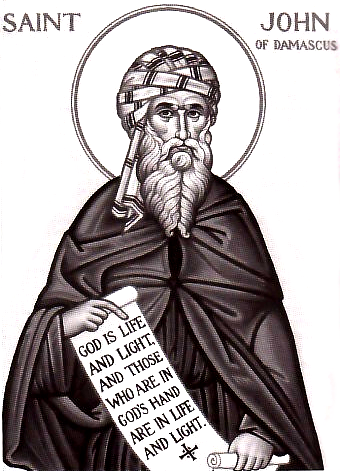
\includegraphics[height=1.67in]{art/damascene}

Ye faithful, come let us honor with songs of praise
the comely sounding and sweet-spoken nightingale,
who doth adorn and captivate the Church of Christ with his sweet songs:
\rubric{John}, the all-wise Damascene, let us honor resplendently,
the divine and eloquent, and the chief of hymnographers;
who verily was filled to the utmost with every divine and earthly wisdom.
\end{center}
\vfill
\cleardoublepage

\setcounter{tocdepth}{1}
\setlength{\cftbeforesecskip}{0em}
\tableofcontents

\cleardoublepage

\pagenumbering{arabic}
\pagestyle{fancyplain}

\parindent=0pt
\parskip=8pt

\section{Preparing to Worship}

\subsection{Trisagion Prayers}

In the Name of the Father, and of the Son, and of the Holy Spirit. Amen.

Glory to thee, our God, glory to thee.

O heavenly King, O Comforter, the Spirit of truth, who art in all places and fillest all things; Treasury of good things and Giver of life: Come and dwell in us and cleanse us from every stain, and save our souls, O gracious Lord.

Holy God, Holy Mighty, Holy Immortal: have mercy on us. \rubric{(thrice)}

Glory to the Father, and to the Son, and to the Holy Spirit: both now and ever and unto ages of ages. Amen.

All-holy Trinity, have mercy on us. Lord, cleanse us from our sins. Master, pardon our iniquities. Holy God, visit and heal our infirmities for thy Name's sake.

Lord, have mercy. \rubric{(thrice)}

Glory to the Father, and to the Son, and to the Holy Spirit: both now and ever, and unto ages of ages. Amen.

Our Father, who art in heaven, hallowed be thy Name; thy kingdom come; thy will be done on earth, as it is in heaven. Give us this day our daily bread; and forgive us our trespasses, as we forgive those who trespass against us; and lead us not into temptation, but deliver us from evil.

Through the prayers of our holy Fathers, Lord Jesus Christ our God, have mercy on us and save us. Amen.

\subsection{Prayer on Entering the Church}

    By the multitude of Thy mercy I will come into Thine house; in Thy fear will I worship toward Thy holy temple. Lead me, O Lord, in Thy righteousness; because of mine enemies, make my way plain before Thee, that with a clear mind I may glorify thee forever, One Divine Power worshiped in three persons: Father, Son, and Holy Spirit. Amen. 

\subsection{Prayer Before the Icon of Christ}

    We reverence thy spotless Icon, O gracious Lord, and ask forgiveness of our transgressions, O Christ our God: for of thine own good will thou wast pleased to ascend the Cross in the flesh, that thou mightest deliver from bondage to the enemy those whom thou hadst fashioned. Wherefore, we cry aloud unto thee: thou hast filled all things with joy, O our Savior, for thou didst come to save the world.

\subsection{Prayer Before the Icon of the Theotokos}

    Forasmuch as thou art a well-spring of tenderness, O Theotokos, make us worthy of compassion; Look upon a sinful people; Manifest thy power as ever, for hoping on thee we cry aloud unto thee: Hail! as once did Gabriel, Chief Captain of the Bodiless Powers.
    
\subsection{Prayer Before Reading Scripture}

Illumine our hearts, O Master who lovest mankind, with the pure light of thy divine knowledge, and open the eyes of our mind to the understanding of thy gospel teachings; implant in us also the fear of thy blessed commandments, that trampling down all carnal desires, we may enter upon a spiritual manner of living, both thinking and doing such things as are well-pleasing unto thee. For thou art the Illumination of our souls and bodies, O Christ our God, and unto thee we ascribe glory, together with thine unoriginate Father and thine all-holy and good and life-giving Spirit, now and ever, and unto ages of ages. Amen.

\subsection{A Prayer Before Reading Spiritual Texts}

O Lord Jesus Christ, open the eyes of my heart, that I may hear thy word and that I may understand and do thy will, for I am a sojourner upon the earth. Hide not thy commandments from me, but open my eyes, that I may perceive the wonders of thy law. Reveal to me the hidden and secret lore of thy wisdom. In thou, O God, do I place my hope. Enlighten my mind and understanding with the light of thy knowledge, not only to cherish those things that are written, but to do them; that in reading the lives and sayings of the saints I may not sin, but that such may serve for my renewal, enlightenment, and sanctification, for the salvation of my soul and the inheritance of everlasting life. For thou art the enlightenment of those who lie in darkness, and from thee cometh every good deed and every gift.
Amen.

\subsection{A Prayer Before Singing}

O Lord, strengthen me to concentrate attentively on the words I pronounce. Grant that these words may come from the depth of my soul. May the vivifying grace of the Holy Spirit pour into the hearts of those who hear our song.

May our prayers become a sweet spiritual fragrance that rises before Thee for all mankind, filled with hope and love for Thee. Grant that we who praise Thee may be united by Thy Holy Spirit in a bond of love, that with one mouth and one heart we might praise, bless, and worship Thee, the Light above all Lights, the True Life, and the Salvation of our souls. Amen.

\cleardoublepage

\section{Selections from Vespers}

\subsection{Psalm 103}

Bless the Lord, O my soul. O Lord my God, thou art very great; thou art clothed with honor and majesty. Who coverest thyself with light as with a garment: who stretchest out the heavens like a curtain: Who layeth the beams of his chambers in the waters: who maketh the clouds his chariot: who walketh upon the wings of the wind: Who maketh his angels spirits; his ministers a flaming fire: Who laid the foundations of the earth, that it should not be removed forever. Thou coveredst it with the deep as with a garment: the waters stood above the mountains. At thy rebuke they fled; at the voice of thy thunder they hasted away. They go up by the mountains; they go down by the valleys unto the place which thou hast founded for them. Thou has set a bound that they may not pass over; that they turn not again to cover the earth. He sendeth the springs into the valleys, which run among the hills. They give drink to every beast of the field; the wild asses quench their thirst. By them shall the fowls of the heaven have their habitation, which sing among the branches. He watereth the hills from his chambers: the earth is satisfied with the fruit of thy works. He causeth the grass to grow for the cattle, and herb for the service of man: that he may bring forth food out of the earth: And wine that maketh glad the heart of man, and oil to make his face to shine, and bread which strengtheneth man's heart. The trees of the Lord are full of sap; the cedars of Lebanon, which he hath planted; Where the birds make their nests: as for the stork, the fir trees are her house. The high hills are a refuge for the wild goats; and the rocks for the conies. He appointed the moon for seasons: the sun knoweth his going down. Thou makest darkness, and it is night: wherein all the beasts of the forest do creep forth. The young lions roar after their prey, and seek their meat from God. The sun ariseth, they gather themselves together, and lay them down in their dens. Man goeth forth unto his work and to his labor until the evening. O Lord, how manifold are thy works! in wisdom hast thou made them all: the earth is full of thy riches. So is this great and wide sea, wherein are things creeping, innumerable, both small and great beasts. There go the ships: there is that Leviathan, whom thou hast made therein. These wait all upon thee; that thou mayest give them their meat in due season. That thou givest them they gather: thou openest thine hand, they are filled with good. Thou hidest thy face, they are troubled: thou takest away their breath, they die, and return to their dust. Thou sendest forth thy spirit, they are created: and thou renewest the face of the earth. The glory of the Lord shall endure forever: the Lord shall rejoice in his works. He looketh on the earth, and it trembleth: he toucheth the hills, and they smoke. I will sing unto the Lord as long as I live: I will sing praise to my God while I have my being. My meditation of him shall be sweet: I will be glad in the Lord. Let the sinners be consumed out of the earth, and let the wicked be no more. Bless thou the Lord, O my soul. Praise ye the Lord.

\subsection{Prayers at the Lighting of the Lamps}
\rubric{(1.)} O Lord, compassionate and merciful, long-suffering and plenteous in mercy, give ear to our prayer, and attend to the voice of our supplication. Work upon us a sign for good. Lead us in thy way, that we may walk in thy truth. Make glad our hearts, that we may fear thy holy name. For thou art great and doest wonders. Thou alone art God, and among all the gods there is none like unto thee, O Lord, mighty in mercy, gracious in strength, to aid and to comfort and to save all those who put their trust in thy holy name. For unto thee are due all glory, honor and worship to the Father and to the Son and to the Holy Spirit, now and ever, and unto ages of ages. Amen.

\rubric{(2.)} O Lord, rebuke us not in thy displeasure, neither chasten us in thy wrath, but deal with us according to thy mercy, O Physician and Healer of our souls. Guide us unto the haven of thy will. Enlighten the eyes of our hearts to the knowledge of thy truth, and vouchsafe that the remainder of this day and our whole life may be peaceful and without sin, through the intercessions of the holy Theotokos and of all the saints. For thine is the might, and thine is the kingdom and the power and the glory of the Father and of the Son and of the Holy Spirit, now and ever, and unto ages of ages. Amen.

\rubric{(3.)} O Lord our God, remember us sinners and thine unprofitable servants when we call upon thy holy name, and put us not to shame in our expectation of thy mercy; but grant us, O Lord, all our petitions which are unto salvation, and vouchsafe that we may love and fear thee with all our hearts and do thy will in all things. For thou art a good God and lovest mankind, and unto thee we ascribe glory to the Father and to the Son and to the Holy Spirit, now and ever, and unto ages of ages. Amen.

\rubric{(4.)} O thou who, with never-silent hymns and never-ceasing songs of praise to thy glory, art hymned by the holy powers: Fill our mouths with thy praise, that we may magnify thy holy name. And grant unto us part and inheritance with all those who fear thee in truth and keep thy commandments, through the intercessions of the holy Theotokos and of all thy saints. For unto thee are due all glory, honor and worship to the Father and to the Son and to the Holy Spirit, now and ever, and unto ages of ages. Amen.

\rubric{(5.)} O Lord, O Lord, who upholdest all things in the undefiled hollow of thy hand, who showest long-suffering upon us all and repentest thee at our wickedness: Remember thy compassions and thy mercy. Visit us with goodness, and grant that, through the remainder of the present day, by thy grace, we may avoid the diverse subtle snares of the evil one and preserve our lives unassailed, through the grace of thine allhly Spirit. Through the mercy and love toward mankind of thine only-begotton Son, with whom thou art blessed, together with thine all-holy and good and life-giving Spirit, now and ever, and unto ages of ages. Amen.

\rubric{(6.)} O God, great and wonderful, who with wisdom inscrutable and great riches of providence orderest all things and bestowest upon us earthly good things, who hast given us a pledge of the promised kingdom through the good things already bestowed upon us and hast made us to shun all evil during that part of the day which is past: Grant that we may also fulfill the remainder of this day without reproach before thy holy glory and hymn thee, the only good One, our God, who lovest mankind. For thou art our God and unto thee we ascribe glory to the Father and to the Son and to the Holy Spirit, now and ever, and unto ages of ages. Amen.

\rubric{(7.)} O great and most high God, who alone hast immortality and dwellest in light unapproachable, who hast made all creation in wisdom, who hast divided the light from the darkness and hast appointed the sun to rule the day, the moon and stars also to rule the night, who hast vouchsafed unto us sinners at this present hour also to come before thy presence with confession and to offer unto thee our evening praise: Do thou thyself, O Lord who lovest mankind, direct our prayer as incense before thee, and accept it as a savour of sweet-smelling fragrance, and grant that we may pass the present evening and the com ing night in peace. Endue us with the armour of light. Deliver us from the terror of the night and from everything that walketh in darkness, and grant that the sleep which thou hast appointed for the repose of our weakness may be free from every imagination of the devil. Yea, O Master of all, Bestower of good things, may we, being moved to compunction upon our beds, call to remembrance thy name in the night, that, enlightened by meditation on thy commandments, we may rise up in joyfulness of soul to glorify thy goodness, offering up unto thy tender love prayers and supplications for our sins and for those of all thy people, whom do thou visit in mercy, through the intercessions of the holy Theotokos. For thou art a good God and lovest mankind, and unto thee we ascribe glory to the Father and to the Son and to the Holy Spirit, now and ever, and unto ages of ages. Amen.

\subsection{Psalm 140}
%\enlargethispage{-\baselineskip} % Widow prevention
O Lord, I have cried out unto thee, hear me: give ear to the voice of my supplication, when I cry out unto thee. Let my prayer be set forth before thee as incense; and the lifting up of my hands as the evening sacrifice.  Set a watch, O Lord, before my mouth and a protecting door about my lips. Incline not my heart to evil words, to make excuses in sins with men that work iniquities, and I will not communicate with the choicest of them. The just man shall correct me in mercy and shall reprove me, but let not the oil of the sinner anoint my head, for my prayer also shall still be against the things with which they are well pleased. Their judges falling upon the rock have been swallowed up. They shall hear my words for they are sweet. As when the thickness of the earth is broken up upon the ground, their bones are scattered by the side of hell. But to thee, O Lord, Lord, are mine eyes. In thee have I put my trust. Take not away my soul. Keep me from the snare which they have laid for me, and the traps of the workers of iniquity. Let the wicked fall into their own nets, while I alone escape.

\subsection{Psalm 141}

I cried unto the Lord with my voice, with my voice unto the Lord did I make my supplication. I poured out my supplication before him, I showed before him my trouble. When my spirit was overwhelmed within me, then thou didst know my path. In the way wherein I walked, have they secretly laid a snare for me. I looked on my right hand and beheld, but there was no one that would know me. Refuge failed me, no one cared for my soul. I cried unto thee, O Lord. I said, Thou art my refuge and my portion in the land of the living. Attend unto my cry, for I am brought very low. Deliver me from my persecutors, for they are stronger than I. Bring my soul out of prison, that I may praise thy name. For the righteous shall wait for me, until thou recompense me.

\subsection{Psalm 129}

Out of the depths have I cried unto thee, O Lord, Lord hear my voice. Let thine ears be attentive to the voice of my supplication.  If thou, O Lord, shouldest mark iniquities, O Lord, who shall stand? For with thee there is forgiveness. Because of thy name have I waited for thee, O Lord. My soul hath waited upon thy word. My soul hath hoped in the Lord. From the morning watch until night, from the morning watch, let Israel trust in the Lord. For with the Lord there is mercy, and with him is abundant redemption, and he shall deliver Israel from all his iniquities.

\subsection{Psalm 116}

Praise the Lord, all ye nations. Praise him all ye people. For his mercy is great toward  us, and the truth of the Lord endureth forever.

\subsection{Phos hilaron}

O Gladsome Light of the holy glory, of the immortal, heavenly, holy, blessed Father, O Jesus Christ: we that come to the setting of the sun, when we behold the evening light, praise Father, Son, and Holy Spirit, God. Meet it is for Thee at all times to be praise with gladsome voices, O Son of God, giver of life; wherefore the whole world doth glorify Thee.

\subsection{Evening Prayer}

Vouchsafe, O Lord, to keep us this night without sin. Blessed art thou, O Lord, the God of our fathers, and praise and glorified is thy Name forever. Amen.

Let thy mercy be upon us, O Lord, even as we have set our hope on thee. Blessed art thou, O Lord; teach me thy statutes. Blessed art thou, O Master; make me to understand thy commandments. Blessed art thou, O Holy One; enlighten me with thy precepts.

Thy mercy, O Lord, endureth forever: O despise not the works of thy hands. To thee belongeth worship, to thee belongeth praise, to thee belongeth glory: to the Father, and to the Son, and to the Holy Spirit: now and ever, and unto ages of ages. Amen.

\subsection{St. Simeon's Prayer}

Lord, now lettest thou thy servant depart in peace, according to thy word: for mine eyes have seen thy salvation, which thou hast prepared before the face of all people; a light to lighten the Gentiles, and the glory of thy people Israel.

\cleardoublepage

\section{Small Compline}

\input{prayers/usualbeginning}

\subsection{Psalm 50}

% source: Antiochian Service Book
Have mercy upon me, O God, according to thy great mercy: according to the multitude of thy tender mercies blot out mine iniquity. Wash me thoroughly from mine iniquity, and cleanse me from my sin. For I acknowledge mine iniquity, and my sin is ever before me. Against thee only have I sinned, and done evil in thy sight: that thou mightest be justified in thy words, and prevail when thou art judged. For behold, I was shapened in iniquity, and in sins did my mother conceive me.  For behold, thou hast loved truth: the unclear and hidden things of thy wisdom thou hast made clear to me. Thou shalt sprinkle me with hyssop, and I shall be clean; thou shalt wash me, and I shall be whiter than snow. Thou shalt make me to hear joy and gladness; the bones which thou hast broken shall rejoice. Turn away thy face from my sins, and blot out all mine iniquities. Create in me a clean heart, O God, and renew a right spirit within me. Cast me not away from thy presence, and take not thy Holy Spirit from me. Restore unto me the joy of thy salvation, and steady me with a guiding spirit.  Then will I teach transgressors thy ways, and the impious shall be converted unto thee. Deliver me from bloodguiltiness, O God, thou God of my salvation, and my tongue shall sing aloud of thy righteousness. O Lord, open thou my lips, and my mouth shall declare thy praise. For hadst thou desired sacrifice, I would have given it thee; thou delightest not in burnt offerings. Sacrifices to God are a contrite spirit: a contrite and humble heart, O God, thou wilt not despise. Do good, O Lord, in thy good will unto Zion, that the walls of Jerusalem may be built up. Then shalt thou be pleased with the sacrifice of righteousness, with burnt offering and whole burnt offerings; Then shall they offer bullocks upon thine altar.


\subsection{Psalm 69}

% source: A Psalter for Prayer
O God, make speed to save me; O Lord, make haste to help me. Let them be ashamed and confounded that seek after my soul. Let them be turned backward and be ashamed that wish me evil. Let them for their reward be soon brought to shame that say over me, Well, well. Let all those that seek Thee be joyful and glad in Thee, O God, and let all such as delight in Thy salvation say always, The Lord be praised. But I am poor and needy, O God; help me! Thou art my helper and my redeemer, O Lord; make no long tarrying.


\subsection{Psalm 142}

% source: Antiochian Service Book
Hear my prayer, O Lord, give ear to my supplications: in thy faithfulness answer me, and in thy righteousness. And enter not into judgment with thy servant: for in thy sight shall no man living be justified. For the enemy hath persecuted my soul; he hath smitten my life down to the ground; he hath made me to dwell in darkness, as those that have been long dead. Therefore is my spirit overwhelmed within me; my heart within me is desolate. I remember the days of old; I meditate on all thy works; I muse on the work of thy hands. I stretch forth my hands unto thee: my soul thirsteth after thee, as a thirsty land. Hear me speedily, O Lord: my spirit faileth: hide not thy face from me, lest I be like unto them that go down into the pit. Cause me to hear thy lovingkindness in the morning; for in thee do I trust: cause me to know the way wherein I should walk; for I lift up my soul unto thee. Deliver me, O Lord, from mine enemies: I flee unto thee to hide me. Teach me to do thy will; for thou art my God: thy spirit is good; lead me into the land of uprightness. Quicken me, O Lord, for thy name's sake: for thy righteousness' sake bring my soul out of trouble. And of thy mercy cut off mine enemies, and destroy all them that afflict my soul: for I am thy servant.


\subsection{The Small Doxology}

Glory be to God on high and on earth peace, and good will among men.

We praise Thee, we bless Thee, we give thanks to Thee for Thy great glory.

O Lord, heavenly King, God the Father Almighty; O Lord the Only-begotten Son Jesus Christ, and the Holy Spirit.

O Lord God, Lamb of God, Son of the Father, that takest away the sin of the world, have mercy on us, Thou that takest away the sins of the world.

Receive our prayer, Thou that sittest at the right hand of the Father, have mercy on us.

For Thou only art holy; Thou only art the Lord, O Jesus Christ, to the glory of God the Father. Amen.

Every day will I bless Thee, and I will praise Thy name for ever, yea, for ever and ever.

Lord, Thou hast been our refuge from all generation. I said: Be merciful unto me; heal my soul for I have sinned against Thee.

Lord, I have fled unto Thee, teach me to do Thy will, for Thou art my God.

For with Thee is the fountain of life; in Thy light shall we see light.

O continue Thy lovingkindness unto them that know Thee.

Vouchsafe, O Lord, to keep us this night without sin.

Blessed art Thou, O Lord God of our Fathers, and praised and glorified be Thy name forever. Amen.

Let Thy mercy, O Lord, be upon us, as we do put our hope in Thee.

Blessed art Thou, O Lord, teach me Thy statutes.

Blessed art Thou, O Master, make me to understand thy commandments.

Blessed art Thou, O Holy One, enlighten me with thy precepts.

Thy mercy, O Lord endureth forever: O despise not the works of Thy hands.

To Thee belongeth worship, to Thee belongeth praise, to Thee belongeth glory, to the Father, and to the Son, and to the Holy Spirit, now and ever, and unto ages of ages. Amen.


\subsection{The Creed}

I believe in one God, the Father Almighty, Maker of heaven and earth, and of all things visible and invisible;

And in one Lord Jesus Christ, the Son of God, the Only-begotten, Begotten of the Father before all worlds, Light of Light, Very God of Very God, Begotten, not made; of one essence with the Father, by whom all things were made:

Who for us men and for our salvation came down from heaven, and was incarnate of the Holy Spirit and the Virgin Mary, and was made man;

And was crucified also for us under Pontius Pilate, and suffered and was buried;

And the third day He rose again, according to the Scriptures;

And ascended into heaven, and sitteth at the right hand of the Father;

And He shall come again with glory to judge the quick and the dead, Whose kingdom shall have no end.

And I believe in the Holy Spirit, the Lord, and Giver of Life, Who proceedeth from the Father, Who with the Father and the Son together is worshiped and glorified, Who spake by the Prophets;

And I believe in One Holy Catholic and Apostolic Church.

I acknowledge one Baptism for the remission of sins.

I look for the Resurrection of the dead.

And the Life of the world to come. Amen.


\subsection{Canon}

\rubric{An appropriate akathist hymn, canon, or other prayers may be said here. The service continues with:}

It is truly meet to bless thee, O Theotokos, ever blessed and all-blameless, and the mother of our God. More honorable than the Cherubim, and more glorious beyond compare than the Seraphim, thou who without stain barest God the Word, and art truly Theotokos, we magnify thee.

\subsection{Trisagion}

Holy God... Glory \rubric{and} Both now... All-holy Trinity... Lord, have mercy. \rubric{(3)}... Glory \rubric{and} Both now... Our Father...

Through the prayers of our holy Fathers, Lord Jesus Christ our God, have mercy on us and save us. Amen.

\subsection{Kontakion}

\rubric{The appointed kontakion or the apolytikion of the great feast or saint being commemorated is now read. If there is no appointed kontakion or commemoration, the following used:}

O God of our fathers, who ever dealest with us according to thy goodness, remove not thy mercy from us; but by their intercessions direct our lives in peace.

In all the world thy Church, arrayed in the blood of thy martyrs as in purple and fine linen, crieth through them unto thee, O Christ our God: Send down thy compassion upon thy people; give peace to thy commonwealth and to our souls great mercy.

Glory to the Father, and to the Son, and to the Holy Spirit.

With the saints give rest, O Christ, to the souls of thy servants, where there is neither sickness nor sorrow nor sighing but life everlasting.

Both now and ever, and unto ages of ages. Amen.

Through the intercessions of all the saints and of the Theotokos, grant us thy peace, O Lord, and have mercy upon us, for thou alone art compassionate.

\rubric{But on Friday evening, use \unrubric{Unto thee, O Lord the Author of creation} and on Saturday evening, use the hypakoe or resurrectional troparion of the proper tone, which can be found starting on page \pageref{resurrectional}.}

\subsection{Prayer of the Hours}

Lord, have mercy. \rubric{(forty times)}

% source: Antiochian Service Book
O Christ our God, who at all times and in every hour, in heaven and on earth, art worshiped and glorified; who art longsuffering, merciful and compassionate; who lovest the just and showest mercy upon the sinner; who callest all to salvation through the promise of blessings to come; O Lord, in this hour receive our supplications, and direct our lives according to thy commandments. Sanctify our souls, hallow our bodies, correct our thoughts, cleanse our minds; deliver us from all tribulation, evil and distress. Encompass us with thy holy Angels, that guided and guarded by them, we may attain to the unity of the faith and to the knowledge of thine unapproachable glory, for thou art blessed unto ages of ages. Amen.


Lord have mercy. \rubric{(thrice)}

Glory to the Father, and to the Son, and to the Holy Spirit: both now and ever, and unto ages of ages. Amen.

More honorable than the Cherubim, and more glorious beyond compare than the Seraphim, thou who without stain barest God the Word, and art truly Theotokos, we magnify thee.

\subsection{Prayer of St. Ephraim the Syrian}

\rubric{If it is Great Lent, say the prayer of St. Ephraim the Syrian and the Trisagion.}

O Lord and Master of my life, take from me the spirit of sloth, meddling, lust of power and idle talk. \rubric{(prostration)}

But give rather the spirit of chastity, humility, patience, and love to thy servant. \rubric{(prostration)}

Yea, O Lord and King, grant me to see my own sins and not to judge my brother, for thou art blessed unto ages of ages. Amen. \rubric{(prostration)}


Holy God... Glory \rubric{and} Both now... All-holy Trinity... Lord, have mercy. \rubric{(3)}... Glory \rubric{and} Both now... Our Father...

Through the prayers of our holy Fathers, Lord Jesus Christ our God, have mercy on us and save us. Amen.

\rubric{The service continues with:}

Lord, have mercy. \rubric{(twelve times)}

\subsection{Prayer of St. Paul of Evergetes}

O spotless, undefiled, incorrupt, immaculate, pure Virgin, Lady Bride of God, who by thy wondrous conceiving hast united God the Word to man, and joined the outcast nature of our race to heavenly things, O only hope of the hopeless, and succor of the embattled, the ready help of them that have recourse to thee, and refuge of all Christians: abhor me not, the sinner, the accursed one, who have altogether made myself unprofitable by shameful thoughts, words, and deeds, and with the heartsease of life's pleasures am become a thrall in mind. But as the Mother of the man-befriending God, do thou, in man-befriending wise, take pity upon me a sinner and prodigal, and receive my supplication, offered thee on unclean lips. And using thy boldness as a mother, entreat thy Son, our Master and Lord, that He may open even unto me the loving compassions of His goodness, and that, overlooking mine innumerable trespasses, He would turn me to repentance, and make me the approved doer of His commandments. And be thou ever with me, as thou art merciful, and compassionate, and the lover of good, being in this life a fervent protectress and help, to defend me from the assaults of adversaries, and guide me unto salvation; and in the hour of my departure, to care for my wretched soul, and drive far from it the dark countenances of evil demons; and in the terrible day of judgment, to deliver me from eternal torment, and show me forth as an heir of the unspeakable glory of thy Son and our God. This be my lot, O my Lady, most holy Theotokos, by thy mediation and help, through the grace and love for man of thine Only-begotten Son, our Lord and God and Savior Jesus Christ, to Whom is due all glory, honor, and worship, with His Father which is without beginning, and His All-holy and good and life-giving Spirit, now and ever, and unto ages of ages. Amen.

\subsection{Prayer of St. Antiochus}

And grant us, O Master, when we go to sleep, repose of body and soul; and keep us from the murky slumbering of sin and every dark voluptuousness of night. Calm the violence of the passions, quench the fiery darts of the evil one, which are treacherously hurled against us. Subdue the rebellions of our flesh, and quell our every earthly and material thought. And grant unto us, O God, a watchful mind, a chaste thought, a sober heart, and sleep light and free from all satanic phantasies. And raise us up at the hour of prayer, established in Thy commandments and holding the remembrance of Thy judgments unshakable within us. Grant us to hymn Thy glory all the night long, that we may praise and bless and glorify Thine all-honored and majestic Name, of the Father, and of the Son, and of the Holy Spirit, now and ever, and unto the ages of ages. Amen.

O most glorious, ever-virgin, blessed Theotokos, present our prayer to thy Son our God, and intercede with him that through thee he may save our souls.

The Father is my Hope; \rubric{(metania)} \\
The Son is my Refuge; \rubric{(metania)} \\
The Holy Spirit is my Protection; \rubric{(metania)}\\
O Holy Trinity: Glory to thee.

In thee, O Mother of God, I place all my hope; keep me under thy protection.

\subsection{Prayer to Our Guardian Angel}

O holy Angel who accompanieth my wretched soul and lowly life, forsake me not, and depart not from me because of my extravagance and wickedness. Give not access to the evil demon to rule with his might this mortal body of mine, but hold me by my wretched, feeble hand; lead me in the path of salvation. Yea, O holy Angel of God, guardian and protector of my wretched soul and body, forgive me all wherewith I have heretofore saddened thee all the days of my life. And though this day I have sinned, be thou my shelter this night. Keep me from all the wiles of the enemy, that I may not anger God with any sin. Intercede with the Lord for me, that he may confirm me in his fear and show me forth as a worthy servant of his goodness. Amen.

Through the prayers of our holy Fathers, Lord Jesus Christ our God, have mercy on us and save us. Amen.

\cleardoublepage

\section{Simplified Midnight Office}

In the Name of the Father, and of the Son, and of the Holy Spirit. Amen.

Glory to thee, our God, glory to thee.

O heavenly King, O Comforter, the Spirit of truth, who art in all places and fillest all things; Treasury of good things and Giver of life: Come and dwell in us and cleanse us from every stain, and save our souls, O gracious Lord.

Holy God... Glory \rubric{and} Both now... All-holy Trinity... Lord, have mercy. \rubric{(3)}... Glory \rubric{and} Both now... Our Father...

Through the prayers of our holy Fathers, Lord Jesus Christ our God, have mercy on us and save us. Amen.

Lord, have mercy. \rubric{(twelve times)}

Glory to the Father, and to the Son, and to the Holy Spirit: both now and ever and unto ages of ages. Amen.

O come, let us worship and fall down before God our King. \rubric{(metania)}

O come, let us worship and fall down before Christ our King and our God. \rubric{(metania)}

O come, let us worship and fall down before Christ Himself, our King and our God. \rubric{(metania)}


\subsection{Psalm 50}

% source: Antiochian Service Book
Have mercy upon me, O God, according to thy great mercy: according to the multitude of thy tender mercies blot out mine iniquity. Wash me thoroughly from mine iniquity, and cleanse me from my sin. For I acknowledge mine iniquity, and my sin is ever before me. Against thee only have I sinned, and done evil in thy sight: that thou mightest be justified in thy words, and prevail when thou art judged. For behold, I was shapened in iniquity, and in sins did my mother conceive me.  For behold, thou hast loved truth: the unclear and hidden things of thy wisdom thou hast made clear to me. Thou shalt sprinkle me with hyssop, and I shall be clean; thou shalt wash me, and I shall be whiter than snow. Thou shalt make me to hear joy and gladness; the bones which thou hast broken shall rejoice. Turn away thy face from my sins, and blot out all mine iniquities. Create in me a clean heart, O God, and renew a right spirit within me. Cast me not away from thy presence, and take not thy Holy Spirit from me. Restore unto me the joy of thy salvation, and steady me with a guiding spirit.  Then will I teach transgressors thy ways, and the impious shall be converted unto thee. Deliver me from bloodguiltiness, O God, thou God of my salvation, and my tongue shall sing aloud of thy righteousness. O Lord, open thou my lips, and my mouth shall declare thy praise. For hadst thou desired sacrifice, I would have given it thee; thou delightest not in burnt offerings. Sacrifices to God are a contrite spirit: a contrite and humble heart, O God, thou wilt not despise. Do good, O Lord, in thy good will unto Zion, that the walls of Jerusalem may be built up. Then shalt thou be pleased with the sacrifice of righteousness, with burnt offering and whole burnt offerings; Then shall they offer bullocks upon thine altar.


\subsection{Psalm 120}

% source: A Psalter for Prayer
I lifted up mine eyes unto the hills; from whence will my help come? My help cometh even from the Lord, Who hath made heaven and earth. Suffer not thy feet to slip, nor Him that keepeth thee to slumber. Behold, He that keepeth Israel shall neither slumber nor sleep. The Lord Himself shall keep thee; the Lord is thy shelter upon thy right hand; The sun shall not burn thee by day, neither the moon by night. The Lord shall keep thee from all evil; yea, the Lord shall preserve thy soul. The Lord shall preserve thy going out, and thy coming in, from this time forth, and for evermore.


\subsection{Psalm 133}

% source: A Psalter for Prayer
Behold now, bless ye the Lord, all ye servants of the Lord, that stand in the house of the Lord, even in the courts of the house of our God. Lift up your hands by night in the sanctuary, and bless the Lord. The Lord bless thee out of Zion, Who hath made heaven and earth.


Glory to the Father, and to the Son, and to the Holy Spirit: both now and ever, and unto ages of ages. Amen.

Alleluia, alleluia, alleluia. Glory to thee, O God. \rubric{(thrice)}

Lord, have mercy. \rubric{(thrice)}

\subsection{Troparia to the Holy Trinity}

Having arisen from sleep, we fall down before thee, O Blessed One, and sing to thee, O Mighty One, the Angelic Hymn: Holy, holy, holy art thou, O God. Through the Theotokos have mercy on us.

Glory to the Father, and to the Son, and to the Holy Spirit:

From my bed and sleep Thou hast raised me: O Lord, enlighten my mind and my heart, and open my lips that I may praise thee, O Holy Trinity: Holy, holy, holy art thou, O God. Through the Theotokos have mercy on us.

Both now and ever, and unto ages of ages. Amen.

Suddenly the Judge shall come, and the deeds of each shall be revealed: but with fear we cry out in the middle of the night: Holy, holy, holy art thou, O God. Through the Theotokos have mercy on us.

\subsection{Prayer to the Holy Trinity}

Arising from sleep I thank thee, O holy Trinity, because of the abundance of thy goodness and longsuffering thou wast not wroth with me, slothful and sinful as I am; neither hast thou destroyed me in my transgressions: but in thy compassion raised me up, as I lay in despair; that at dawn I might sing the glories of thy Majesty. Do thou now enlighten the eyes of my understanding, open my mouth to receive thy words, teach me thy commandments, help me to do thy will, confessing thee from my heart, singing and praising thine All-holy Name: of the Father, and of the Son, and of the Holy Spirit: now and ever, and unto ages of ages. Amen.

\subsection{The Creed}

I believe in one God, the Father Almighty, Maker of heaven and earth, and of all things visible and invisible;

And in one Lord Jesus Christ, the Son of God, the Only-begotten, Begotten of the Father before all worlds, Light of Light, Very God of Very God, Begotten, not made; of one essence with the Father, by whom all things were made:

Who for us men and for our salvation came down from heaven, and was incarnate of the Holy Spirit and the Virgin Mary, and was made man;

And was crucified also for us under Pontius Pilate, and suffered and was buried;

And the third day He rose again, according to the Scriptures;

And ascended into heaven, and sitteth at the right hand of the Father;

And He shall come again with glory to judge the quick and the dead, Whose kingdom shall have no end.

And I believe in the Holy Spirit, the Lord, and Giver of Life, Who proceedeth from the Father, Who with the Father and the Son together is worshiped and glorified, Who spake by the Prophets;

And I believe in One Holy Catholic and Apostolic Church.

I acknowledge one Baptism for the remission of sins.

I look for the Resurrection of the dead.

And the Life of the world to come. Amen.


\subsection{A Prayer of St. Basil}

We bless thee, O God most high and Lord of mercies, who ever workest great and mysterious deeds for us, glorious, wonderful, and numberless; who providest us with sleep as a rest from our infirmities and as a repose for our bodies tired by labor. We thank thee that thou hast not destroyed us in our transgressions, but in thy love toward mankind thou hast raised us up, as we lay in despair, that we may glorify thy Majesty. We entreat thine infinite goodness, enlighten the eyes of our understanding and raise up our minds from the heavy sleep of indolence; open our mouths and fill them with thy praise, that we may unceasingly sing and confess thee, who art God glorified in all and by all, the eternal Father, the Only-Begotten Son, and the all-holy and good and life-giving Spirit: now and ever, and unto ages of ages. Amen.
%\enlargethispage{-2\baselineskip} % Widow prevention

O most glorious, ever-virgin, blessed Theotokos, present our prayer to thy Son our God, and intercede with him that through thee he may save our souls.

The Father is my Hope; \rubric{(metania)}\\
The Son is my Refuge; \rubric{(metania)}\\
The Holy Spirit is my Protection; \rubric{(metania)}\\
O Holy Trinity: Glory to thee.

In thee, O Mother of God, I place all my hope; keep me under thy protection.

It is truly meet to bless thee, O Theotokos, ever blessed and all-blameless, and the mother of our God. More honorable than the Cherubim, and more glorious beyond compare than the Seraphim, thou who without stain barest God the Word, and art truly Theotokos, we magnify thee.

O Lord who lovest mankind, forgive those who hate and wrong us. Do good to those who do good. Grant our brethren and kindred their petitions leading unto salvation and eternal life. Visit the sick and grant them healing. Guide those at sea. Journey with those who travel. Struggle alongside the Orthodox. To those who serve and are kind to us, grant remission of sins.

On Thy servants \rubric{(names of the living)}, and on those who have charged us, unworthy as we are, to pray for them, have mercy according to Thy great mercy. Remember, O Lord, Thy servants \rubric{(names of the departed)}, our fathers and brethren who have fallen asleep, and grant them rest where the light of Thy countenance shines. Remember, O Lord, those who bear fruit and do good works in Thy holy churches and grant them their petitions leading unto salvation and eternal life. Remember also, O Lord, us, Thy humble, sinful and unworthy servants, and enlighten our minds with the light of Thy knowledge, and guide us in the way of Thy commandments, by the prayers of our immaculate Lady, the Theotokos, and Ever-Virgin Mary, and of all Thy Saints, for Thou art blessed to the ages of ages. Amen. 

\subsection{Prayer of St. Ephraim the Syrian}

\rubric{If it is Great Lent, say the prayer of St. Ephraim the Syrian.}

O Lord and Master of my life, take from me the spirit of sloth, meddling, lust of power and idle talk. \rubric{(prostration)}

But give rather the spirit of chastity, humility, patience, and love to thy servant. \rubric{(prostration)}

Yea, O Lord and King, grant me to see my own sins and not to judge my brother, for thou art blessed unto ages of ages. Amen. \rubric{(prostration)}


\rubric{Lastly, we say:}

Through the prayers of our holy Fathers, Lord Jesus Christ our God, have mercy on us and save us. Amen.

\cleardoublepage

\section{The Six Psalms and Orthros Prayers}

\subsection{Psalm 3}

Lord, how are they increased that trouble me! Many are they that rise up against me. Many there be which say of my soul, There is no help for him in God. But thou, O Lord, art a shield for me; my glory, and the lifter up of mine head. I cried unto the Lord with my voice, and he heard me out of his holy hill. I laid me down and slept; I awaked; for the Lord sustained me. I will not be afraid of ten thousands of people, that have set themselves against me round about. Arise, O Lord; save me, O my God: for thou hast smitten all mine enemies upon the cheek bone; thou hast broken the teeth of the ungodly. Salvation belongeth unto the Lord: thy blessing is upon thy people.

\subsection{Psalm 37}

O Lord, rebuke me not in thy wrath: neither chasten me in thy hot displeasure. For thine arrows stick fast in me, and thy hand presseth me sore. There is no soundness in my flesh because of thine anger; neither is there any rest in my bones because of my sin. For mine iniquities are gone over mine head: as an heavy burden they are too heavy for me. My wounds stink and are corrupt because of my foolishness. I am troubled; I am bowed down greatly; I go mourning all the day long. For my loins are filled with a loathsome disease: and there is no soundness in my flesh. I am feeble and sore broken: I have roared by reason of the disquietness of my heart. Lord, all my desire is before thee; and my groaning is not hid from thee. My heart panteth, my strength faileth me: as for the light of mine eyes, it is also gone from me. My lovers and my friends stand aloof from my sore; and my kinsmen stand afar off. They also that seek after my life lay snares for me: and they that seek my hurt speak mischievous things, and imagine deceits all the day long. But I, as a deaf man, heard not; and I was as a dumb man that openeth not his mouth. Thus I was as a man that heareth not, and in whose mouth are no reproofs. For in thee, O Lord, do I hope: thou wilt hear, O Lord my God. For I said, Hear me, lest otherwise they should rejoice over me: when my foot slippeth, they magnify themselves against me. For I am ready to halt, and my sorrow is continually before me. For I will declare mine iniquity; I will be sorry for my sin. But mine enemies are lively, and they are strong: and they that hate me wrongfully are multiplied. They also that render evil for good are mine adversaries; because I follow the thing that good is. Forsake me not, O Lord: O my God, be not far from me. Make haste to help me, O Lord my salvation.

\subsection{Psalm 62}

O God, thou art my God; early will I seek thee: my soul thirsteth for thee, my flesh longeth for thee in a dry and thirsty land, where no water is; to see thy power and thy glory, so as I have seen thee in the sanctuary. Because thy lovingkindness is better than life, my lips shall praise thee. Thus will I bless thee while I live: I will left up my hands in thy name. My soul shall be satisfied as with marrow and fatness; and my mouth shall praise thee with joyful lips: when I remember thee upon my bed, and meditate on thee in the night watches. Because thou hast been my help, therefore in the shadow of thy wings will I rejoice. My soul followeth hard after thee: thy right hand upholdeth me. But those that seek after my soul, to destroy it, shall go into the lower parts of the earth. They shall fall by the sword: they shall be a portion for foxes. But the king shall rejoice in God; everyone that sweareth by him shall glory: but the mouth of them that speak lies shall be stopped.

\subsection{Psalm 87}

O Lord God of my salvation, I have cried day and night before thee: let my prayer come before thee: incline thine ear unto my cry; for my soul is full of troubles: and my life draweth nigh unto the grave. I am counted with them that go down into the pit: I am as a man that hath no strength: free among the dead, like the slain that lie in the grave, whom thou rememberest no more: and they are cut off from thy hand. Thou hast laid me in the lowest pit, in darkness, in the deeps. Thy wrath lieth hard upon me, and thou hast afflicted me with all thy waves. Thou hast put away mine acquaintance far from me: thou hast made me an abomination unto them: i am shut up, and I cannot come forth. Mine eye mourneth by reason of affliction: Lord, I have called daily upon thee, I have stretched out my hands unto thee. Wilt thou shew wonders to the dead? shall the dead arise and praise thee? Shall thy lovingkindess be declared in the grave? or thy faithfulness in destruction? Shall thy wonders be known in the dark? and thy righteousness in the land of forgetfulness? But unto thee have I cried, O Lord; and in the morning shall my prayer come before thee. Lord, why castest thou off my soul? why hidest thou thy face from me? I am afflicted and ready to die from my youth up: while I suffer thy terrors I am distracted. Thy fierce wrath goeth over me: thy terrors have cut me off. They came round about me daily like water; they compassed me about together. Lover and friend hast thou put far from me, and mine acquaintance into darkness.

\subsection{Psalm 102}

Bless the Lord, O my soul: and all that is within me, bless his holy name. Bless the Lord, O my soul, and forget not all his benefits: who forgiveth all thine iniquities; who healeth all thy diseases; who redeemeth thy life from destruction; who crowneth thee with lovingkindness and tender mercies; who satisfieth thy mouth with good things; so that thy youth is renewed like the eagle's. The Lord executeth righteousness and judgment for all that are oppressed. He made known his ways unto Moses, his acts unto the children of Israel. The Lord is merciful and gracious, slow to anger, and plenteous in mercy. He will not always chide: neither will he keep his anger forever. He hath not dealt with us after our sins; nor rewarded us according to our iniquities. For as the heaven is high above the earth, so great is his mercy toward them that fear him. As far as the east is from the west, so far hath he removed our transgressions from us. Like as a father pitieth his children, so the Lord pitieth them that fear him. For he knoweth our frame; he remembereth that we are dust. As for man, his days are as grass: as a flower of the field, so he flourisheth. For the wind passeth over it, and it is gone; and the place thereof shall know it no more. But the mercy of the Lord is from everlasting to everlasting upon them that fear him, and his righteousness unto children's children; to such as keep his covenant, and to those that remember his commandments to do them. The Lord hath prepared his throne in the heavens; and his kingdom ruleth over all. Bless the Lord, ye his angels, that excel in strength, that do his commandments, hearkening unto the voice of his word. Bless ye the Lord, all ye his hosts; ye ministers of his, that do his pleasure. Bless the Lord, all his works in all places of his dominion: bless the Lord, O my soul.

\subsection{Psalm 142}

Hear my prayer, O Lord, give ear to my supplications: in thy faithfulness answer me, and in thy righteousness. And enter not into judgment with thy servant: for in thy sight shall no man living be justified. For the enemy hath persecuted my soul; he hath smitten my life down to the ground; he hath made me to dwell in darkness, as those that have been long dead. Therefore is my spirit overwhelmed within me; my heart within me is desolate. I remember the days of old; I meditate on all thy works; I muse on the work of thy hands. I stretch forth my hands unto thee: my soul thirsteth after thee, as a thirsty land. Hear me speedily, O Lord: my spirit faileth: hide not thy face from me, lest I be like unto them that go down into the pit. Cause me to hear thy lovingkindness in the morning; for in thee do I trust: cause me to know the way wherein I should walk; for I lift up my soul unto thee. Deliver me, O Lord, from mine enemies: I flee unto thee to hide me. Teach me to do thy will; for thou art my God: thy spirit is good; lead me into the land of uprightness. Quicken me, O Lord, for thy name's sake: for thy righteousness' sake bring my soul out of trouble. And of thy mercy cut off mine enemies, and destroy all them that afflict my soul: for I am thy servant.

\subsection{The Twelve Orthros Prayers}

\rubric{(1.)} We give thanks unto thee, O Lord our God, who hast raised us up from our beds and hast put into our mouths a word of praise, that we may worship and call upon thy holy name. And we entreat thee, by thy mercies which thou hast exercised always in our life, send down now also thine aid upon those who stand before the face of thy holy glory and await the rich mercy which is from thee. And grant that they may always, with fear and love, adore thee, praise thee, hymn thee and worship thine inexpressible goodness. For unto thee are due all glory, honor and worship to the Father and to the Son and to the Holy Spirit, now and ever, and unto ages of ages. Amen.

\rubric{(2.)} Out of the night our spirit awaketh at dawn unto thee, O our God; for thy commandments are a light upon the earth. Teach us to perfect righteousness and holiness in thy fear; for we glorify thee, our God, who dost truly exist. Incline thine ear, and hear us, and be mindful, O Lord of the names of all those who are with us and pray with us, and save them by thy might. Bless thy people, and sanctify thine inheritance. Give peace to thy world, to thy churches, to the priests, to all civil authorities and all thy people. For blessed and glorified is thine all-honorable and majestic name of the Father and of the Son and of the Holy Spirit, now and ever and unto ages of ages. Amen.

\rubric{(3.)} Out of the night our spirit awaketh at dawn unto thee, O God; for thy commandments are a light. Teach us thy righteousness, thy commandments and thy statues, O God. Enlighten the eyes of our understanding lest at any time we sleep unto death in sins. Dispel all darkness from our hearts. Graciously give unto us the Sun of righteousness, and by thy Holy Spirit preserve our life unassailed. Guide our steps into the way of peace. Grant us to behold the dawn and the day with joy, that we may raise our morning prayers unto thee. For thine is the might, and thine is the kingdom and the power and the glory of the Father and of the Son and of the Holy Spirit, now and ever, and unto ages of ages. Amen.

\rubric{(4.)} O Master God, holy and unsearchable, who didst command the light to shine forth from the darkness, who hast refreshed us by the slumber of the night and hast raised us up to glorify and supplicate thy goodness: Being implored of thine own tender loving-kindness, receive us also now who worship thee and render thanks unto thee according to the measure of our strength; and grant us all our petitions which are unto salvation. Make us sons of the light and of the day and heirs of thine everlasting good things. Be mindful, O Lord, in the multitude of thy mercies, of all thy people here present with us and who pray with us and all our brethren on land, on the sea, in the air and in every place of thy dominion, who are in need of thy love for mankind and of thy help, and grant unto all thy great mercy, that being preserved in safety of soul and body, we may with boldness magnify thy wondrous and blessed name of the Father and of the Son and of the Holy Spirit, now and ever, and unto ages of ages. Amen.

\rubric{(5.)} O Treasury of good things, Fountain eternal, O holy Father who workest wonders, allpowerful and almighty: We worship thee and pray thee, calling thy mercies and thy compassions to the aid and defense of our lowliness. Be mindful of thy servants, O Lord; receive the morning prayers of us all as incense before thee; and let none of us be found reprobate, but encompass us with thy compassions. Be mindful, O Lord, of those who watch and sing to the glory of thine only-begotten Son, who is our God, and thy Holy Spirit. Be thou their Helper and their Support. Receive thou their supplications upon thy most heavenly and ideal altar. For thou art our God, and unto thee we ascribe glory to the Father and to the Son and to the Holy Spirit, now and ever, and unto ages of ages. Amen.

\rubric{(6.)} We give thanks unto thee, O Lord God of our salvation; for thou doest all things which are for the welfare of our souls, that we may ever look upward unto thee, the Saviour and Benefactor of our souls. For thou hast refreshed us in that part of the night which is past and hast raised us up from our beds and hast led us to stand here in worship of thy precious name. Wherefore we entreat thee, O Lord, give us grace and power, that we may be vouchsafed with understanding to sing praise unto thee and to pray without ceasing, in fear and trembling working out our own salvation, through the help of thy Christ. Be mindful, O Lord, of those who cry aloud unto thee in the night; hearken unto them, and have mercy, and crush under their feet invisible and warring enemies. For thou art the King of peace and the Saviour of our souls, and unto thee we ascribe glory to the Father and to the Son and to the Holy Spirit, now and ever, and unto ages of ages. Amen.

\rubric{(7.)} O God and Father of our Lord Jesus Christ, who hast raised us up from our beds and hast gathered us together at this hour of prayer: Grant us grace in the opening of our mouth, and receive our thanksgivings as we have power to make them, and instruct us in thy statutes. For we know not how to pray as we ought unless thou, O Lord, by thy Holy Spirit, dost guide us. Wherefore, we beseech thee: Forgive, remit, pardon whatsoever sins we may have committed unto this present hour, whether by word or deed or thought, whether voluntarily or involuntarily; for if thou wilt be extreme to mark iniquity, O Lord, Lord, who shall stand? For with thee is redemption. For thou only art holy, a mighty Helper and the Defender of our life, and our song shall ever be of thee. Blessed and glorified be the might of thy kingdom of the Father and of the Son and of the Holy Spirit, now and ever, and unto ages of ages. Amen.

\rubric{(8.)} O Lord our God, who hast banished from us the sluggishness of sleep and hast called us together by a holy bidding, that in the night also we may lift up our hands and confess thy righteous judgments: Receive our prayers, petitions, confessions and nocturnal adoration and grant unto us, O God, faith unashamed, hope unwavering, love unfeigned. Bless our comings and our goings, our deeds and works and words and thoughts. And grant that we may come to the beginning of this day praising, singing and blessing the goodness of thine ineffable beneficence. For blessed is thine all-holy name, and glorified is thy kingdom of the Father and of the Son and of the Holy Spirit, now and ever, and unto ages of ages. Amen.

\rubric{(9.)} Illumine our hearts, O Master who lovest mankind, with the pure light of thy divine knowledge, and open the eyes of our mind to the understanding of thy gospel teachings; implant in us also the fear of thy blessed commandments, that trampling down all carnal desires, we may enter upon a spiritual manner of living, both thinking and doing such things as are well-pleasing unto thee. For thou art our Sanctification and Illumination, and unto thee we ascribe glory to the Father and to the Son and to the Holy Spirit, now and ever, and unto ages of ages. Amen.

\rubric{(10.)} O Lord our God, who hast granted unto men pardon through repentance and hast set for us the repentance of the prophet David as an example of the acknowledgement of sin and of confession which is unto forgiveness: Do thou thyself, O Master, have mercy on us according to thy great mercy, notwithstanding the manifold and great iniquities into which we have fallen; and according to the multitude of thy compassions, blot out our transgressions. Against thee have we sinned, O Lord, thou who knowest the hidden and secret things in the heart of men and who alone hast power to forgive sins; and as thou hast created a clean heart within us and established us with thy governing Spirit and made known unto us the joy of thy salvation, cast us not away from thy presence. But inasmuch as thou art good and lovest mankind, graciously vouchsafe that even until our uttermost breath, we may offer unto thee the sacrifice of righteousness and an oblation upon thy holy altar. Through the mercy and compassions and love for mankind of thine only-begotten Son, with whom thou art blessed, together with thine all-holy and good and life-giving Spirit, now and ever, and unto ages of ages. Amen.

\rubric{(11.)} O God, our God, who hast brought into being by thy will all the powers endowed with speech and reason, we pray thee and supplicate thee: Receive our praise, which together with all thy creatures we offer according to our strength, and reward us with the rich gifts of thy goodness. For unto thee every knee doth bow, whether in heaven or on earth or in the regions under the earth, and every breath and created being doth sing thine ineffable glory, for thou only art the true and most merciful God. For all the powers of heaven praise thee, and unto thee they ascribe glory to the Father and to the Son and to the Holy Spirit, now and ever, and unto ages of ages. Amen.

\rubric{(12.)} We praise thee, we hymn thee, we bless thee, we give thanks unto thee, O God of our fathers, that thou hast brought us in safety through the shades of night and hast shown unto us once again the light of day. And we entreat of thy goodness: Be gracious unto our sins, and receive our prayer in thy great tenderness. For we flee unto thee, the merciful and almighty God. Illumine our hearts with the true Sun of thy righteousness; enlighten our mind and guard all our senses, that walking uprightly as in the day, in the way of thy commandments, we may attain unto life eternal, for with thee is the fountain of life, and may graciously be vouchsafed to come unto the fruition of the light unapproachable. For thou art our God, and unto thee we ascribe glory to the Father and to the Son and to the Holy Spirit, now and ever, and unto ages of ages. Amen.

\section{First Hour}

In the Name of the Father, and of the Son, and of the Holy Spirit. Amen.

Glory to thee, our God, glory to thee.

O heavenly King, O Comforter, the Spirit of truth, who art in all places and fillest all things; Treasury of good things and Giver of life: Come and dwell in us and cleanse us from every stain, and save our souls, O gracious Lord.

Holy God... Glory \rubric{and} Both now... All-holy Trinity... Lord, have mercy. \rubric{(3)}... Glory \rubric{and} Both now... Our Father...

Through the prayers of our holy Fathers, Lord Jesus Christ our God, have mercy on us and save us. Amen.

Lord, have mercy. \rubric{(twelve times)}

Glory to the Father, and to the Son, and to the Holy Spirit: both now and ever and unto ages of ages. Amen.

O come, let us worship and fall down before God our King. \rubric{(metania)}

O come, let us worship and fall down before Christ our King and our God. \rubric{(metania)}

O come, let us worship and fall down before Christ Himself, our King and our God. \rubric{(metania)}

\subsection{Psalm 5}

Hear my words, O Lord; consider my cry. Attend unto the voice of my supplication, my King, and my God, for unto Thee will I pray, O Lord. Early in the morning shalt Thou hear my voice; early in the morning will I stand before Thee, and Thou shalt watch over me. For Thou art a God that hast no pleasure in wickedness; the evil-doer shall not dwell nigh Thee. Such as be lawless shall not stand in Thy sight, for Thou hatest all them that work iniquity. Thou shalt destroy all them that speak lies; the Lord will abhor the blood-thirsty and deceitful man. But as for me, by the multitude of Thy mercy I will come into Thine house; in Thy fear will I worship toward Thy holy temple. Lead me, O Lord, in Thy righteousness; because of mine enemies, make my way plain before Thee. For there is no truth in their mouth; their heart is vain; their throat is an open sepulcher; they flatter with their tongue. Judge them, O God; let them fall through their own imaginations; cast them out according to the multitude of their ungodliness; for they have embittered Thee, O Lord. And let all them that put their trust in Thee be glad; they shall ever rejoice; and Thou shalt dwell in them and they that love Thy Name shall be joyful in Thee. For Thou wilt bless the righteous, O Lord, for with the shield of Thy favorable kindness hast Thou crowned us.

\subsection{Psalm 89}

Lord, Thou hast been our refuge from generation to generation. Before ever the mountains were formed, or the earth and the world were created, even from age to age Thou art. Turn not man away unto humiliation; yea, Thou hast said, Be converted, ye children of men. For a thousand years before Thine eyes, O Lord, are but as yesterday when it is past, and as a watch in the night. Fleeting shall their years be; he shall go by in the morning like the grass; in the morning it shall flourish, and grow up, but in the evening it shall fall away, and dry up, and wither. For we consumed away in Thy displeasure, and were troubled at Thy wrathful indignation. Thou hast set our misdeeds before Thee, our years are in the light of Thy countenance. For all our days are spent, and we have disappeared in Thy wrath; Our years are spun out like a spider’s web. The days of our age are threescore years and ten, or if we be so strong, fourscore years, and more than these is but labor and sorrow; for frailty shall come upon us, and we shall be chastened. Who knoweth the power of Thy wrath, and from fear of Thee, who can recount Thine anger? So make Thy right hand known to me, and to them that are bound by the heart in wisdom. Turn Thee again, O Lord; how long? And be gracious unto Thy servants. We were satisfied with Thy mercy in the morning, O Lord, and we rejoiced and were glad; We were glad all our days; for the days wherein Thou didst humble us, the years wherein we saw adversity. And look upon Thy servants, and upon Thy works, and guide their children, and let the brightness of the Lord our God be upon us, and prosper Thou the work of our hands upon us; yea, prosper Thou our handy-work.

\subsection{Psalm 100}

Mercy and judgment shall be my song unto Thee, O Lord; I sing and understand in a blameless way; when wilt Thou come unto me? I have walked in the innocency of my heart in the midst of my house. I have set no unlawful thing before mine eyes; I have hated the workers of iniquity. A froward heart hath not cleaved unto me; I did not know the crafty man that turned away from me. Whoso privily slandereth his neighbor, him did I drive out; whoso hath a proud look and a greedy stomach, with such I did not eat. Mine eyes look upon such as are faithful in the land, that they may dwell with me; whoso leadeth a godly life, he shall be my servant. The proud doer hath not dwelt in the midst of my house; he that speaketh unjustly shall have no place in my sight. In the morning I slew all the sinners of the land, to consume all the workers of lawlessness from the city of the Lord.

Glory to the Father, and to the Son, and to the Holy Spirit: both now and ever, and unto ages of ages. Amen.

Alleluia, alleluia, alleluia. Glory to thee, O God. \rubric{(thrice)}

Lord, have mercy. \rubric{(thrice)}

\subsection{Troparia and Verses}

\rubric{If it is a weekday of Great Lent, the following troparia and verses are sung in Tone 6, else we say \unrubric{Glory...}, the troparion of the day, then \unrubric{Both now...}. The troparion of the day can be found starting on page \pageref{weekday}.}

Glory to the Father, and to the Son, and to the Holy Spirit: both now and ever, and unto ages of ages. Amen.

In the morning attend unto the voice of my supplication, O my King and my God. \rubric{(prostration)}

\rubric{Verse 1:} Unto my words give ear, O Lord; hear my cry. \rubric{(prostration)}

\rubric{Verse 2:} For unto thee will I pray, O Lord: thou shalt hearken in the morning to my voice. \rubric{(prostration)}

Glory to the Father, and to the Son, and to the Holy Spirit: both now and ever, and unto ages of ages. Amen.

\subsection{Theotokion and Psalm Verses}

What shall I call thee, O thou who art full of grace? Heaven, for from thee shone forth the Sun of righteousness; Paradise, for thou hast budded forth the Flower of immortality; Virgin, for thou hast remained incorrupt; Pure Mother, for thou hast held in thy holy embrace a Son, who is God of all. Beseech thou him to save our souls.

My steps do thou direct according to thy saying, and so let no iniquity have dominion over me. \rubric{(twice in Lent)}

Deliver me from the false accusation of men, and I will keep thy commandments. \rubric{(twice in Lent)}

Make thy face to shine upon thy servant, and teach me thy statutes. \rubric{(twice in Lent)}

Let my mouth be filled with thy praise, O Lord, that I may hymn thy glory and thy majesty all the day long. \rubric{(thrice in Lent)}

\subsection{Trisagion}

Holy God... Glory \rubric{and} Both now... All-holy Trinity... Lord, have mercy. \rubric{(3)}... Glory \rubric{and} Both now... Our Father...

Through the prayers of our holy Fathers, Lord Jesus Christ our God, have mercy on us and save us. Amen.

\subsection{Kontakion}

\rubric{The kontakion of the day can be found starting on page \pageref{weekday}. If it is Great Lent, use the following kontakia:}

\rubric{Monday, Tuesday, Thursday:} With hearts and mouths let us continually magnify the glorious Mother of God, more holy than the angels, confessing her to be the Theotokos, who did, in very truth, bring forth God incarnate and who unceasingly doth intercede for our souls.

\rubric{Wednesday, Friday:} Quickly go before us, O Christ our God, lest the enemy which blasphemeth thee and constraineth us, lead us into captivity. Overcome by the cross those who war against us, that they may know what power hath the faith of Orthodox believers; through the intercessions of the Theotokos, O thou who alone lovest mankind.

\rubric{Saturday:} Unto thee, O Lord, the Author of creation, the universe doth offer the God-bearing martyrs as the first-fruits of nature. By whose prayers, through the Theotokos, do thou preserve thy Church in profound peace, O most merciful One.

\rubric{On Sunday, use the hypakoe of the proper tone, which can be found starting on page \pageref{resurrectional}.}

\subsection{Prayer of the Hours}

Lord, have mercy. \rubric{(forty times)}

O Christ our God, who at all times and in every hour, in heaven and on earth, art worshiped and glorified; who art longsuffering, merciful and compassionate; who lovest the just and showest mercy upon the sinner; who callest all to salvation through the promise of blessings to come; O Lord, in this hour receive our supplications, and direct our lives according to thy commandments. Sanctify our souls, hallow our bodies, correct our thoughts, cleanse our minds; deliver us from all tribulation, evil and distress. Encompass us with thy holy Angels, that guided and guarded by them, we may attain to the unity of the faith and to the knowledge of thine unapproachable glory, for thou art blessed unto ages of ages. Amen.

Lord have mercy. \rubric{(thrice)}

Glory to the Father, and to the Son, and to the Holy Spirit: both now and ever, and unto ages of ages. Amen.

More honorable than the Cherubim, and more glorious beyond compare than the Seraphim, thou who without stain barest God the Word, and art truly Theotokos, we magnify thee.

\subsection{Prayer of St. Ephraim the Syrian}

\rubric{If it is Great Lent, say the prayer of St. Ephraim the Syrian and the Trisagion.}

O Lord and Master of my life, take from me the spirit of sloth, meddling, lust of power and idle talk. \rubric{(prostration)}

But give rather the spirit of chastity, humility, patience, and love to thy servant. \rubric{(prostration)}

Yea, O Lord and King, grant me to see my own sins and not to judge my brother, for thou art blessed unto ages of ages. Amen. \rubric{(prostration)}

Holy God... Glory \rubric{and} Both now... All-holy Trinity... Lord, have mercy. \rubric{(3)}... Glory \rubric{and} Both now... Our Father...

Through the prayers of our holy Fathers, Lord Jesus Christ our God, have mercy on us and save us. Amen.

Lord, have mercy. \rubric{(twelve times)}

\subsection{The Final Prayer}

O Christ, the true Light, which illumineth and sanctifieth every man who cometh into the world: Let the light of thy countenance be signed upon us, that in it we may behold the light unapproachable. Guide our footsteps aright, to the keeping of thy commandments, through the intercessions of thine all-immaculate Mother and of all thy saints. Amen.

Through the prayers of our holy Fathers, Lord Jesus Christ our God, have mercy on us and save us. Amen.

\cleardoublepage

\section{Third Hour}

In the Name of the Father, and of the Son, and of the Holy Spirit. Amen.

Glory to thee, our God, glory to thee.

O heavenly King, O Comforter, the Spirit of truth, who art in all places and fillest all things; Treasury of good things and Giver of life: Come and dwell in us and cleanse us from every stain, and save our souls, O gracious Lord.

Holy God... Glory \rubric{and} Both now... All-holy Trinity... Lord, have mercy. \rubric{(3)}... Glory \rubric{and} Both now... Our Father...

Through the prayers of our holy Fathers, Lord Jesus Christ our God, have mercy on us and save us. Amen.

Lord, have mercy. \rubric{(twelve times)}

Glory to the Father, and to the Son, and to the Holy Spirit: both now and ever and unto ages of ages. Amen.

O come, let us worship and fall down before God our King. \rubric{(metania)}

O come, let us worship and fall down before Christ our King and our God. \rubric{(metania)}

O come, let us worship and fall down before Christ Himself, our King and our God. \rubric{(metania)}

\subsection{Psalm 16}

Hear my just cause, O Lord; attend unto my supplication. Hearken unto my prayer, that goeth not out of flattering lips. From Thy presence shall my judgment come forth; let mine eyes look upon the things that are right. Thou hast proved my heart; Thou hast visited in the night. Thou hast tried me, and unrighteousness hath not been found within me. That my mouth shall not speak of men’s works, for the sake of the words of Thy lips I have kept hard ways. O hold Thou up my goings in Thy paths, that my footsteps slip not. I called, for Thou hast heard me, O God; incline Thine ear to me, and hearken unto my words. Make Thy mercies marvelous, Thou that art the Savior of them which put their trust in Thee, from such as resist Thy right hand. Keep me, O Lord, as the apple of Thine eye; hide me under the shelter of Thy wings, from the presence of the ungodly that trouble me; mine enemies compass my soul round about. They are enclosed in their own fat, and their mouth speaketh proud things. They that cast me out have now surrounded me; they have turned their eyes down to the ground, like as a lion that is greedy of his prey, and as it were a lion’s whelp, lurking in secret places. Arise, O Lord, disappoint them, and trip them up; deliver my soul from the ungodly, Thy sword from the enemies of Thy hand. O Lord, divide them in their life from the few of the earth; yea, from Thy hid treasure hath their belly been filled. They had children at their desire, and left the rest of their substance for their babes. But as for me, in righteousness shall I appear before Thy face; when Thy glory is revealed, I shall be satisfied.

\subsection{Psalm 24}

Unto thee, O Lord, have I lifted up my soul; my God, I have put my trust in Thee: O let me never be confounded, neither let mine enemies laugh me to scorn; for all they that wait on Thee shall not be ashamed. Let them be ashamed such as transgress without a cause. Tell me Thy ways, O Lord, and teach me Thy paths. Lead me forth unto Thy truth, and teach me, for Thou art God my Savior, and upon Thee have I waited all the day long; remember Thy loving-kindnesses, O Lord, and Thy mercies, which are from everlasting. O remember not the sins of my youth, and of mine ignorance; according to Thy mercy think Thou upon me, O Lord, for Thy goodness’ sake. Gracious and righteous is the Lord, therefore will He give a Law to sinners in the way. He will guide the meek unto judgment, He shall teach the meek His ways. All the paths of the Lord are mercy and truth unto such as keep His covenant, and His testimonies. For Thy Name’s sake, O Lord, be merciful unto my sin, for it is great. What man is he, that feareth the Lord? To him shall He give a Law in the way which He hath chosen. His soul shall dwell at ease, and his seed shall inherit the land. The Lord is the strength of them that fear Him, and He will show them His covenant. Mine eyes are ever toward the Lord, for He shall pluck my feet out of the net. Be charitable unto me, and have mercy on me, for I am only-begotten and poor. The sorrows of my heart are enlarged; O bring Thou me out of my troubles. Look upon my humbleness and my hardship, and forgive all my sins. Consider mine enemies, how many they are, and they bear a tyrannous hate against me. O keep my soul, and deliver me; let me not be confounded, for I have put my trust in Thee. The innocent and the upright have cleaved unto me, for I waited upon Thee, O Lord. Deliver Israel, O God, out of all his troubles.

\subsection{Psalm 50}

Have mercy upon me, O God, according to thy great mercy: according to the multitude of thy tender mercies blot out mine iniquity. Wash me thoroughly from mine iniquity, and cleanse me from my sin. For I acknowledge mine iniquity, and my sin is ever before me. Against thee only have I sinned, and done evil in thy sight: that thou mightest be justified in thy words, and prevail when thou art judged. For behold, I was shapened in iniquity, and in sins did my mother conceive me.  For behold, thou hast loved truth: the unclear and hidden things of thy wisdom thou hast made clear to me. Thou shalt sprinkle me with hyssop, and I shall be clean; thou shalt wash me, and I shall be whiter than snow. Thou shalt make me to hear joy and gladness; the bones which thou hast broken shall rejoice. Turn away thy face from my sins, and blot out all mine iniquities. Create in me a clean heart, O God, and renew a right spirit within me. Cast me not away from thy presence, and take not thy Holy Spirit from me. Restore unto me the joy of thy salvation, and steady me with a guiding spirit.  Then will I teach transgressors thy ways, and the impious shall be converted unto thee. Deliver me from bloodguiltiness, O God, thou God of my salvation, and my tongue shall sing aloud of thy righteousness. O Lord, open thou my lips, and my mouth shall declare thy praise. For hadst thou desired sacrifice, I would have given it thee; thou delightest not in burnt offerings. Sacrifices to God are a contrite spirit: a contrite and humble heart, O God, thou wilt not despise. Do good, O Lord, in thy good will unto Zion, that the walls of Jerusalem may be built up. Then shalt thou be pleased with the sacrifice of righteousness, with burnt offering and whole burnt offerings; Then shall they offer bullocks upon thine altar.

Glory to the Father, and to the Son, and to the Holy Spirit: both now and ever, and unto ages of ages. Amen.

Alleluia, alleluia, alleluia. Glory to thee, O God. \rubric{(thrice)}

Lord, have mercy. \rubric{(thrice)}

\subsection{Troparia and Verses}

\rubric{If it is a weekday of Great Lent, the following troparia and verses are sung in Tone 6, else we say \unrubric{Glory...}, the troparion of the day, then \unrubric{Both now...}. The troparion of the day can be found starting on page \pageref{weekday}.}

Glory to the Father, and to the Son, and to the Holy Spirit: both now and ever, and unto ages of ages. Amen.

\rubric{If it is a weekday of Great Lent, the following troparia and verses are sung in Tone 6, else we say \unrubric{Glory...}, the troparion of the day, then \unrubric{Both now...}}

Glory to the Father, and to the Son, and to the Holy Spirit: both now and ever, and unto ages of ages. Amen.

O Lord, who at the third hour didst send down upon thine apostles thy Holy Spirit: Take not the same from us, O good One, but renew him in us who pray unto thee. \rubric{(prostration)}

\rubric{Verse 1:} Create in me a clean heart, O God, and renew a right spirit within me. \rubric{(prostration)}

\rubric{Verse 2:} Cast me not away from thy presence, and take not thy Holy Spirit from me. \rubric{(prostration)}

Glory to the Father, and to the Son, and to the Holy Spirit: both now and ever, and unto ages of ages. Amen.

\subsection{Theotokion and Psalm Verses}

O Theotokos, thou art the true vine who didst bud forth for us the Fruit of life. Implore thou him, we beseech thee, O Lady, together with the apostles and all the saints, that he will have mercy on our souls.

Blessed is the Lord God, blessed is the Lord day by day; the God of our salvation shall prosper us along the way. Our God is the God of salvation.

\subsection{Trisagion}

Holy God... Glory \rubric{and} Both now... All-holy Trinity... Lord, have mercy. \rubric{(3)}... Glory \rubric{and} Both now... Our Father...

Through the prayers of our holy Fathers, Lord Jesus Christ our God, have mercy on us and save us. Amen.

\subsection{Kontakion}

\rubric{The kontakion of the day can be found starting on page \pageref{weekday}. If it is Great Lent, say:}

Blessed art thou, O Christ our God, who hast revealed the fishermen as all-wise by sending down upon them the Holy Spirit; through them thou didst draw the world into thy net. O Lover of mankind, glory to thee.

Glory to the Father, and to the Son, and to the Holy Spirit.

Grant speedy and steadfast consolation unto thy servants, O Jesus, when our spirits are cast down within us. Depart not from our souls in affliction. Be not far from our thoughts in time of trouble, but always defend us. Draw near unto us, draw near unto us, thou who art everywhere present. As thou art ever with thine apostles, so, also, O compassionate One, unite thyself unto those who long for thee, that with one accord we may sing praises unto thee and glorify thine all-holy Spirit.

Both now and ever, and unto ages of ages. Amen.

The hope and protection and refuge of Christians art thou, the impregnable wall and the haven unvexed by storms, O immaculate Theotokos; but in that thou dost save the world by thine unceasing intercessions, call thou us also to remembrance, O all-lauded Virgin.

\rubric{But on Saturday, use \unrubric{Unto thee, O Lord the Author of creation} and on Sunday, use the hypakoe of the proper tone, which can be found starting on page \pageref{resurrectional}.}

\subsection{Prayer of the Hours}

Lord, have mercy. \rubric{(forty times)}

O Christ our God, who at all times and in every hour, in heaven and on earth, art worshiped and glorified; who art longsuffering, merciful and compassionate; who lovest the just and showest mercy upon the sinner; who callest all to salvation through the promise of blessings to come; O Lord, in this hour receive our supplications, and direct our lives according to thy commandments. Sanctify our souls, hallow our bodies, correct our thoughts, cleanse our minds; deliver us from all tribulation, evil and distress. Encompass us with thy holy Angels, that guided and guarded by them, we may attain to the unity of the faith and to the knowledge of thine unapproachable glory, for thou art blessed unto ages of ages. Amen.

Lord have mercy. \rubric{(thrice)}

Glory to the Father, and to the Son, and to the Holy Spirit: both now and ever, and unto ages of ages. Amen.

More honorable than the Cherubim, and more glorious beyond compare than the Seraphim, thou who without stain barest God the Word, and art truly Theotokos, we magnify thee.

\subsection{Prayer of St. Ephraim the Syrian}

\rubric{If it is Great Lent, say the prayer of St. Ephraim the Syrian and the Trisagion.}

O Lord and Master of my life, take from me the spirit of sloth, meddling, lust of power and idle talk. \rubric{(prostration)}

But give rather the spirit of chastity, humility, patience, and love to thy servant. \rubric{(prostration)}

Yea, O Lord and King, grant me to see my own sins and not to judge my brother, for thou art blessed unto ages of ages. Amen. \rubric{(prostration)}

Holy God... Glory \rubric{and} Both now... All-holy Trinity... Lord, have mercy. \rubric{(3)}... Glory \rubric{and} Both now... Our Father...

Through the prayers of our holy Fathers, Lord Jesus Christ our God, have mercy on us and save us. Amen.

Lord, have mercy. \rubric{(twelve times)}

\subsection{The Final Prayer}

O Master God, Almighty Father, O Lord, the only-begotten Son Jesus Christ, and O Holy Spirit, one Godhead and one Power: Have mercy on me a sinner; and by the judgments which thou hast established, save me, thine unworthy servant, for thou art blessed unto ages of ages. Amen.

Through the prayers of our holy Fathers, Lord Jesus Christ our God, have mercy on us and save us. Amen.

\cleardoublepage

\include{sext}
\section{Ninth Hour}

\input{prayers/usualbeginning}

\subsection{Psalm 83}

% source: A Psalter for Prayer
How amiable are Thy dwellings, O Lord of hosts! My soul desireth and longeth for the courts of the Lord; my heart and my flesh have rejoiced in the living God. Yea, the sparrow hath found her an house, and the dove a nest where she may lay her young, even Thy altars, O Lord of hosts, my King and my God. Blessed are they that dwell in Thy house, for ever and ever will they praise Thee. Blessed is the man whose help is from Thee, in his heart he hath proposed ascents into the valley of tears, unto the place which he hath appointed, for the law-giver shall give the blessing. They will go from strength to strength; the God of gods shall appear in Zion. O Lord God of hosts, hear my prayer; hearken, O God of Jacob. Behold, O God, our defender, and look upon the face of Thy Christ. For one day in Thy courts is better than a thousand; I have preferred to be a doorkeeper in the house of my God, than to dwell in the tents of sinners. For the Lord loveth mercy and truth, God will give grace and glory; the Lord shall withhold no good thing from them that walk innocently. O Lord God of hosts, blessed is the man that putteth his trust in Thee.


\subsection{Psalm 84}

% source: A Psalter for Prayer
Thou hast been gracious, O Lord, unto Thy land, Thou hast turned back the captivity of Jacob. Thou hast forgiven the offenses of Thy people; Thou hast covered all their sins. Thou hast curtailed all Thy displeasure; Thou hast relented from the wrath of Thine indignation. Convert us, then, O God of our salvation, and let Thine anger cease from us. Wilt Thou be displeased at us for ever? Or wilt Thou stretch out Thy wrath from one generation to another? O God, Thou shalt stay Thyself; Thou shalt revive us, and Thy people shall rejoice in Thee. Show us, O Lord, Thy mercy, and grant us Thy salvation. I will hear what the Lord God will say concerning me; for He shall speak peace unto His people, and to His saints, and to them that turn their hearts unto Him. Surely His salvation is nigh them that fear Him, that glory may dwell in our land. Mercy and truth are met together, justice and peace have kissed each other. Truth hath flourished out of the earth, and justice hath looked down from heaven. For the Lord shall show loving-kindness, and our land shall give her increase. Justice shall go before Him, and shall set His steps in the way.


\subsection{Psalm 85}

% source: A Psalter for Prayer
Bow down Thine ear, O Lord, and hear me, for I am poor and in misery. Preserve Thou my soul, for I am holy; save Thy servant, O my God, that putteth his trust in Thee. Have mercy upon me, O Lord, for I will call upon Thee all day. Give joy to the soul of Thy servant, for unto Thee have I lifted up my soul. For Thou, Lord, art good and gentle, and of great mercy unto all them that call upon Thee. Give ear, Lord, unto my prayer, and heed the voice of my supplication. In the day of my trouble I called upon Thee, for Thou hast heard me. Among the gods there is none like unto Thee, O Lord, nor are there any deeds according unto Thy deeds. All nations whom Thou hast made shall come and bow down before Thee, O Lord, and shall glorify Thy Name. For Thou art great, and doest wondrous things; Thou art God alone. Guide me, O Lord, in Thy way, and I will walk in Thy truth; O let my heart rejoice to fear Thy Name. I will thank Thee, O Lord my God, with all my heart, and I will praise Thy Name for evermore. For great is Thy mercy toward me, and Thou hast delivered my soul from the nethermost hell. O God, the wicked are risen against me, and the congregations of the mighty have sought after my soul, and have not set Thee before them. But Thou, O Lord my God, art compassionate and merciful, longsuffering, and greatly charitable and true. O look upon me, and have mercy upon me, give Thy strength unto Thy servant, and help the son of Thine handmaid. Work some sign upon me for good, that they who hate me may see, and be ashamed, because Thou, Lord, hast holpen me, and comforted me.


Glory to the Father, and to the Son, and to the Holy Spirit: both now and ever, and unto ages of ages. Amen.

Alleluia, alleluia, alleluia. Glory to thee, O God. \rubric{(thrice)}

Lord, have mercy. \rubric{(thrice)}

\subsection{Troparia and Verses}

\rubric{If it is a weekday of Great Lent, the following troparia and verses are sung in Tone 8, else we say \unrubric{Glory...}, the troparion of the day, then \unrubric{Both now...}. The troparion of the day can be found starting on page \pageref{weekday}.}

Glory to the Father, and to the Son, and to the Holy Spirit: both now and ever, and unto ages of ages. Amen.

O thou, who at the ninth hour, for our sake didst taste death in the flesh: Mortify thou the pride of our flesh, and save us, O Christ God. \rubric{(prostration)}

\rubric{Verse 1:} Let my supplication draw nigh before thee, O Lord; according to thine oracle give me understanding. \rubric{(prostration)}

\rubric{Verse 2:} Let my petition come before thee, O Lord: according to thine oracle deliver me. \rubric{(prostration)}

Glory to the Father, and to the Son, and to the Holy Spirit: both now and ever, and unto ages of ages. Amen.

\subsection{Theotokion and Psalm Verses}

Thou who for our sake wast born of a virgin and didst suffer crucifixion, O good One, and didst despoil death through death and as God didst reveal resurrection: Despise not those whom thou hast created with thine own hand; show forth thy love for mankind, O merciful One; accept the intercession of thy mother, the Theotokos, for us, and save thy despairing people, O our Savior.

Deliver us not up utterly, for thy holy name's sake, neither disannul thou thy covenant, and cause not thy mercy to depart from us, for Abraham's sake, thy beloved, and for Isaac's sake, thy servant, and for Israel's, thy holy one. 

\subsection{Trisagion}

Holy God... Glory \rubric{and} Both now... All-holy Trinity... Lord, have mercy. \rubric{(3)}... Glory \rubric{and} Both now... Our Father...

Through the prayers of our holy Fathers, Lord Jesus Christ our God, have mercy on us and save us. Amen.

\subsection{Kontakion}

\rubric{The kontakion of the day can be found starting on page \pageref{weekday} for weekdays. If it is Great Lent, say:}

When the thief beheld the Author of life hanging upon the cross, he said: If thou wert not god, who art here crucified with us, then had the sun not veiled its rays, neither would the earth have shaken with trembling. But do thou, who sufferest for all men, remember me, O Lord, when thou comest in thy kingdom.

Glory to the Father, and to the Son, and to the Holy Spirit.

In the midst, between two thieves, was thy cross found, the balance-beam of righteousness; for while the one was led down to hades by the heaviness of his blaspheming, the other was lightened of his sins, unto the knowledge of things divine, O Christ God, glory to thee.

Both now and ever, and unto ages of ages. Amen.

When she who bare thee beheld upon the cross thee, the Lamb and Shepherd and Savior of the world, she weeping said: The world rejoiceth, in that it hath received redemption, but my inward parts are inflamed as I behold thy crucifixion, which thou sufferest for all men, O my Son and my God.

\rubric{But on Saturday, use \unrubric{Unto thee, O Lord the Author of creation} and on Sunday, use the hypakoe of the proper tone, which can be found starting on page \pageref{resurrectional}.}

\subsection{Prayer of the Hours}

Lord, have mercy. \rubric{(forty times)}

O Christ our God, who at all times and in every hour, in heaven and on earth, art worshiped and glorified; who art longsuffering, merciful and compassionate; who lovest the just and showest mercy upon the sinner; who callest all to salvation through the promise of blessings to come; O Lord, in this hour receive our supplications, and direct our lives according to thy commandments. Sanctify our souls, hallow our bodies, correct our thoughts, cleanse our minds; deliver us from all tribulation, evil and distress. Encompass us with thy holy Angels, that guided and guarded by them, we may attain to the unity of the faith and to the knowledge of thine unapproachable glory, for thou art blessed unto ages of ages. Amen.

Lord have mercy. \rubric{(thrice)}

Glory to the Father, and to the Son, and to the Holy Spirit: both now and ever, and unto ages of ages. Amen.

More honorable than the Cherubim, and more glorious beyond compare than the Seraphim, thou who without stain barest God the Word, and art truly Theotokos, we magnify thee.

\subsection{Prayer of St. Ephraim the Syrian}

\rubric{If it is Great Lent, say the prayer of St. Ephraim the Syrian and the Trisagion.}

O Lord and Master of my life, take from me the spirit of sloth, meddling, lust of power and idle talk. \rubric{(prostration)}

But give rather the spirit of chastity, humility, patience, and love to thy servant. \rubric{(prostration)}

Yea, O Lord and King, grant me to see my own sins and not to judge my brother, for thou art blessed unto ages of ages. Amen. \rubric{(prostration)}


Holy God... Glory \rubric{and} Both now... All-holy Trinity... Lord, have mercy. \rubric{(3)}... Glory \rubric{and} Both now... Our Father...

Through the prayers of our holy Fathers, Lord Jesus Christ our God, have mercy on us and save us. Amen.

Lord, have mercy. \rubric{(twelve times)}

\subsection{The Final Prayer}

O Master, Lord Jesus Christ our God, who art longsuffering toward our sins and who hast led us even to the present hour, in which, as thou didst hang upon the life-giving tree thou didst make a way into paradise for the penitent thief and by death didst destroy death: Be gracious unto us sinners and thine unworthy servants; for we have sinned and have dealt iniquitously, and we are not worthy to lift up our eyes and look upon the heights of heaven, inasmuch as we have departed from the path of thy righteousness and have walked after the desires of our own hearts. But we implore of thy boundless goodness: Spare us, O Lord, according to the multitude of thy mercy, and save us, for thy holy name's sake; for our days have passed away in vanity. Wrest us out of the hand of the adversary, and forgive our sins, and mortify our carnal imagination, that, putting off the old man, we may be clothed upon with the new man and may live unto thee, our Master and our Benefactor, and that, so following after thy commandments, we may attain unto rest eternal, where is the abode of all those who rejoice. For thou art, in verity, the true Joy and Exultation of those who love thee, O Christ our God, and unto thee we ascribe glory, together with thine unoriginate Father and thine all-holy and good and life-giving Spirit, now and ever, and unto ages of ages. Amen.

Through the prayers of our holy Fathers, Lord Jesus Christ our God, have mercy on us and save us. Amen.

\cleardoublepage

\section{Typika}

In the Name of the Father, and of the Son, and of the Holy Spirit. Amen.

Glory to thee, our God, glory to thee.

O heavenly King, O Comforter, the Spirit of truth, who art in all places and fillest all things; Treasury of good things and Giver of life: Come and dwell in us and cleanse us from every stain, and save our souls, O gracious Lord.

Holy God... Glory \rubric{and} Both now... All-holy Trinity... Lord, have mercy. \rubric{(3)}... Glory \rubric{and} Both now... Our Father...

Through the prayers of our holy Fathers, Lord Jesus Christ our God, have mercy on us and save us. Amen.

Lord, have mercy. \rubric{(twelve times)}

Glory to the Father, and to the Son, and to the Holy Spirit: both now and ever and unto ages of ages. Amen.

\subsection{Psalm 102}

\rubric{(Tone 8)} Bless the Lord, O my soul: and all that is within me, bless his holy name. Bless the Lord, O my soul, and forget not all his benefits: who forgiveth all thine iniquities; who healeth all thy diseases; who redeemeth thy life from destruction; who crowneth thee with lovingkindness and tender mercies; who satisfieth thy mouth with good things; so that thy youth is renewed like the eagle's. The Lord executeth righteousness and judgment for all that are oppressed. He made known his ways unto Moses, his acts unto the children of Israel. The Lord is merciful and gracious, slow to anger, and plenteous in mercy. He will not always chide: neither will he keep his anger forever. He hath not dealt with us after our sins; nor rewarded us according to our iniquities. For as the heaven is high above the earth, so great is his mercy toward them that fear him. As far as the east is from the west, so far hath he removed our transgressions from us. Like as a father pitieth his children, so the Lord pitieth them that fear him. For he knoweth our frame; he remembereth that we are dust. As for man, his days are as grass: as a flower of the field, so he flourisheth. For the wind passeth over it, and it is gone; and the place thereof shall know it no more. But the mercy of the Lord is from everlasting to everlasting upon them that fear him, and his righteousness unto children's children; to such as keep his covenant, and to those that remember his commandments to do them. The Lord hath prepared his throne in the heavens; and his kingdom ruleth over all. Bless the Lord, ye his angels, that excel in strength, that do his commandments, hearkening unto the voice of his word. Bless ye the Lord, all ye his hosts; ye ministers of his, that do his pleasure. Bless the Lord, all his works in all places of his dominion: bless the Lord, O my soul.

\subsection{Psalm 145}

\rubric{(Tone 2)} Glory to the Father, and to the Son, and to the Holy Spirit.

Praise the Lord, O my soul; While I live will I praise the Lord; I will sing unto my God as long as I have being. O put not your trust in princes, in the sons of men, in whom there is no salvation. His spirit shall go forth, and he shall return again to his earth; in that day all his thoughts shall perish. Blessed is he that hath the God of Jacob for his helper, whose hope is in the Lord his God; Who made heaven and earth, the sea, and all that therein is, Who preserveth truth for ever; Who rendereth judgment for the wronged, Who giveth food unto the hungry; the Lord looseth the fettered; The Lord giveth wisdom to the blind; the Lord raiseth up the fallen; the Lord loveth the righteous; The Lord preserveth the proselytes; He defendeth the fatherless and the widow, but the way of sinners shall He destroy. The Lord shall reign for ever, Thy God, O Zion, unto generation and generation.

\subsection{O Only-Begotten}

Both now and ever and unto ages of ages. Amen.

O only-begotten Son and immortal Word of God, who for our salvation didst will to be incarnate, of the holy Theotokos and ever-virgin Mary and without change didst become man and wast crucified, O Christ our God, trampling down Death by death, who art one of the Holy Trinity, glorified with the Father and the Holy Spirit: Save us.

\subsection{The Beatitudes in Tone Eight}

In thy kingdom remember us, O Lord, when thou comest in thy kingdom.

Blessed are the poor in spirit, for theirs is the kingdom of heaven.

Blessed are those who mourn, for they shall be comforted.

Blessed are the meek, for they shall inherit the earth.

Blessed are those who hunger and thirst for righteousness, for they shall be satisfied.

Blessed are the merciful, for they shall obtain mercy.

Blessed are the pure in heart, for they shall see God.

Blessed are the peacemakers, for they shall be called the sons of God.

Blessed are those who are persecuted for righteousness' sake, for theirs is the kingdom of heaven.

Blessed are you when men revile you and persecute you and utter all kinds of evil against you falsely on my account.

Rejoice and be glad, for your reward is great in heaven.

Glory to the Father, and to the Son, and to the Holy Spirit.

Both now and ever, and unto ages of ages. Amen.

\subsection{The Readings}

\rubric{The appointed epistle and gospel readings are now read, not intoned, from a Bible. Each reading is simply introduced and read, the usual congregational responses being omitted.}

\subsection{Troparia and Verses}

The heavenly choir singeth thy praises, saying: Holy, holy, holy, Lord of Sabaoth; heaven and earth are full of thy glory.

Come unto him, and be enlightened, and your faces shall not be ashamed.

The heavenly choir singeth thy praises, saying: Holy, holy, holy, Lord of Sabaoth; heaven and earth are full of thy glory.

Glory to the Father, and to the Son, and to the Holy Spirit.

The choir of the holy angels and archangels, with all the powers of heaven, singeth thy praises, saying: Holy, holy, holy, Lord of Sabaoth; heaven and earth are full of thy glory.

Both now and ever, and unto ages of ages. Amen.

\subsection{The Creed}

I believe in one God, the Father Almighty, Maker of heaven and earth, and of all things visible and invisible;

And in one Lord Jesus Christ, the Son of God, the Only-begotten, Begotten of the Father before all worlds, Light of Light, Very God of Very God, Begotten, not made; of one essence with the Father, by whom all things were made:

Who for us men and for our salvation came down from heaven, and was incarnate of the Holy Spirit and the Virgin Mary, and was made man;

And was crucified also for us under Pontius Pilate, and suffered and was buried;

And the third day He rose again, according to the Scriptures;

And ascended into heaven, and sitteth at the right hand of the Father;

And He shall come again with glory to judge the quick and the dead, Whose kingdom shall have no end.

And I believe in the Holy Spirit, the Lord, and Giver of Life, Who proceedeth from the Father, Who with the Father and the Son together is worshiped and glorified, Who spake by the Prophets;

And I believe in One Holy Catholic and Apostolic Church.

I acknowledge one Baptism for the remission of sins.

I look for the Resurrection of the dead.

And the Life of the world to come. Amen.

Forgive, remit, pardon, O God, our sins, both voluntary and involuntary, in deed and in word, in knowledge or in ignorance, committed by night or by day, in mind and in thought. Forgive us them all, for thou art good and lovest mankind.

Our Father, who art in heaven, hallowed be thy Name; thy kingdom come; thy will be done on earth, as it is in heaven. Give us this day our daily bread; and forgive us our trespasses, as we forgive those who trespass against us; and lead us not into temptation, but deliver us from evil.

Through the prayers of our holy Fathers, Lord Jesus Christ our God, have mercy on us and save us. Amen.

\subsection{Prayer of the Hours}

Lord, have mercy. \rubric{(forty times)}

O Christ our God, who at all times and in every hour, in heaven and on earth, art worshiped and glorified; who art longsuffering, merciful and compassionate; who lovest the just and showest mercy upon the sinner; who callest all to salvation through the promise of blessings to come; O Lord, in this hour receive our supplications, and direct our lives according to thy commandments. Sanctify our souls, hallow our bodies, correct our thoughts, cleanse our minds; deliver us from all tribulation, evil and distress. Encompass us with thy holy Angels, that guided and guarded by them, we may attain to the unity of the faith and to the knowledge of thine unapproachable glory, for thou art blessed unto ages of ages. Amen.

Lord have mercy. \rubric{(thrice)}

Glory to the Father, and to the Son, and to the Holy Spirit: both now and ever, and unto ages of ages. Amen.

More honorable than the Cherubim, and more glorious beyond compare than the Seraphim, thou who without stain barest God the Word, and art truly Theotokos, we magnify thee.

Through the prayers of our holy Fathers, Lord Jesus Christ our God, have mercy on us and save us. Amen.

Blessed be the name of the Lord, henceforth and forevermore. \rubric{(thrice with metanias)}

\subsection{Psalm 33}

I will bless the Lord at all times, His praise is ever in my mouth. In the Lord shall my soul be praised; let the meek hear, and be glad. O magnify the Lord with me, and we shall exalt His Name together. I sought the Lord and He heard me, yea, He delivered me out of all my troubles. Come unto Him, and be enlightened, and your faces shall not be ashamed. This poor man cried and the Lord heard him, and saved him out of all his troubles. The angel of the Lord tarrieth round about them that fear Him, and delivereth them. O taste, and see, that the Lord is good; blessed is the man that trusteth in Him. O fear the Lord, all ye that are His saints, for they that fear Him lack nothing. The rich have lacked, and suffered hunger, but they that seek the Lord shall want no manner of thing that is good. Come, ye children, and hearken unto me; I will teach you the fear of the Lord. What man is he that lusteth to live, and would gladly see good days? Keep thy tongue from evil, and thy lips, that they speak no guile. Shun evil, and do good; seek peace, and pursue it. The eyes of the Lord are over the righteous, and His ears are open unto their prayers. But the countenance of the Lord is against them that do evil, to root out the remembrance of them from the earth. The righteous cried, and the Lord heard them, and delivered them out of all their troubles. The Lord is nigh unto them that are of a contrite heart, and will save such as be of an humble spirit. Many are the troubles of the righteous, but the Lord delivereth them out of all. The Lord keepeth all their bones; not one of them shall be broken. The death of sinners is evil, and they that hate the righteous shall sin greatly. The Lord will deliver the souls of His servants, and all they that put their trust in Him shall do no sin.

Glory to the Father, and to the Son, and to the Holy Spirit: both now and ever, and unto ages of ages. Amen.

It is truly meet to bless thee, O Theotokos, ever blessed and all-blameless, and the mother of our God. More honorable than the Cherubim, and more glorious beyond compare than the Seraphim, thou who without stain barest God the Word, and art truly Theotokos, we magnify thee.

\subsection{Synaxarion}

\rubric{The appropriate synaxarion readings for the day may optionally be read now, followed by a brief spiritual message if someone has been blessed to give one, or an appropriate reading from a Church Father or other Orthodox text. Any necessary announcements should be made, then the service concludes with:}

Through the prayers of our holy Fathers, Lord Jesus Christ our God, have mercy on us and save us. Amen.

\cleardoublepage

\section{Prayers at the Table}

\subsection{Before Meals}

In the Name of the Father, and of the Son, and of the Holy Spirit. Amen.

Our Father, who art in heaven, hallowed be thy Name; thy kingdom come; thy will be done on earth, as it is in heaven. Give us this day our daily bread; and forgive us our trespasses, as we forgive those who trespass against us; and lead us not into temptation, but deliver us from evil.

For thine is the kingdom, and the power, and the glory, of the Father, and of the Son, and of the Holy Spirit: now and ever, and unto ages of ages. Amen.

Glory to the Father, and to the Son, and to the Holy Spirit: both now and ever, and unto ages of ages. Amen.

Lord, have mercy. \rubric{(thrice)}

\rubric{Then}

    O Christ our God, bless the food and drink of thy servants, for thou art Holy always; now and ever, and unto ages of ages. Amen.

\rubric{Or}

    They that hunger shall eat and be satisfied, they that seek after the Lord shall praise him; their hearts shall live forever. Amen.

\rubric{Or}

    Bless us, O Lord, and these thy gifts of which we are about to partake, for thou art blessed and glorified; now and ever, and unto ages of ages. Amen.

\subsection{After Meals}

Glory to the Father, and to the Son, and to the Holy Spirit: both now and ever, and unto ages of ages. Amen.

Lord, have mercy. \rubric{(thrice)}

\rubric{Then}

    Blessed is God, who is merciful unto us and nourisheth us from His bounteous gifts by His Grace and compassion, always, now and ever, and unto ages of ages. Amen.

\rubric{Or}

    We thank thee, O Christ our God, that thou hast satisfied us with thy earthly gifts, deprive us not of thy Heavenly Kingdom; but as thou entered into the midst of thy disciples, O Savior, and gave them peace, enter also among us and save us. Amen.

\rubric{Or}

    We thank thee, O God, the Giver of all good things, for these gifts and all thy mercies, and we bless thy Holy Name, always, now and ever, and unto ages of ages. Amen.

\cleardoublepage

\section{Prayers of Intercession}

\subsection{Prayer to One's Patron Saint}

Pray unto God for me, O Holy Saint \rubric{(name of patron saint)}, well-pleasing to God: for I turn unto thee, who art the speedy helper and intercessor for my soul.

\subsection{Prayer to One's Guardian Angel}

O Angel of Christ, holy guardian and protector of my soul and body,
forgive me everything wherein I have offended thee every day of my life,
and protect me from all influence and temptation of the evil one. May I
nevermore anger God by any sin. Pray for me to the Lord, that He may
make me worthy of the grace of the All-holy Trinity, and of the Most
Blessed Theotokos, and of all the Saints. Amen.

\subsection{Another Prayer to One's Guardian Angel}

O holy Angel who accompanieth my wretched soul and lowly life, forsake me not, and depart not from me because of my extravagance and wickedness. Give not access to the evil demon to rule with his might this mortal body of mine, but hold me by my wretched, feeble hand; lead me in the path of salvation. Yea, O holy Angel of God, guardian and protector of my wretched soul and body, forgive me all wherewith I have heretofore saddened thee all the days of my life. And though this day I have sinned, be thou my shelter this night. Keep me from all the wiles of the enemy, that I may not anger God with any sin. Intercede with the Lord for me, that he may confirm me in his fear and show me forth as a worthy servant of his goodness. Amen.

\subsection{General Intercession}

O Lord who lovest mankind, forgive those who hate and wrong us. Do good to those who do good. Grant our brethren and kindred their petitions leading unto salvation and eternal life. Visit the sick and grant them healing. Guide those at sea. Journey with those who travel. Struggle alongside the Orthodox. To those who serve and are kind to us, grant remission of sins.

On Thy servants \rubric{(names of the living)}, and on those who have charged us, unworthy as we are, to pray for them, have mercy according to Thy great mercy. Remember, O Lord, Thy servants \rubric{(names of the departed)}, our fathers and brethren who have fallen asleep, and grant them rest where the light of Thy countenance shines. Remember, O Lord, those who bear fruit and do good works in Thy holy churches and grant them their petitions leading unto salvation and eternal life. Remember also, O Lord, us, Thy humble, sinful and unworthy servants, and enlighten our minds with the light of Thy knowledge, and guide us in the way of Thy commandments, by the prayers of our immaculate Lady, the Theotokos, and Ever-Virgin Mary, and of all Thy Saints, for Thou art blessed to the ages of ages. Amen. 

\cleardoublepage

\subsection{Living}

\cleardoublepage

\subsection{Departed}

\cleardoublepage

\section{Litanies}

\subsection{The Litany of Peace}

In peace, let us pray to the Lord.

For the peace from above and the salvation of our souls, let us pray to the Lord.

For the peace of the whole world, the good estate of the holy churches of God and the union of all men, let us pray to the Lord.

For this holy house and those who with faith, reverence, and fear of God enter therein, let us pray to the Lord.

For our metropolitan, \rubric{(name)}, our bishop, \rubric{(name)}, the honorable presbytery; the diaconate in Christ, all the clergy and the people, let us pray to the Lord.

For our president, civil authorities, and armed forces, let us pray to the Lord.

For this city \rubric{(or \unrubric{countryside} or \unrubric{village})} and every city and countryside and the faithful who dwell therein, let us pray to the Lord.

For healthful seasons, abundance of the fruits of the earth and peaceful times, let us pray to the Lord.

For travelers by sea, by land, and by air, the sick, the suffering, the captive, and for their salvation, let us pray to the Lord.

For our deliverance from all tribulation, wrath, danger, and necessity, let us pray to the Lord.

Help us; save us; have mercy on us; and keep us, O God, by thy grace.

Calling to remembrance our all-holy, immaculate, most blessed and glorious Lady the Theotokos and ever-virgin Mary, with all the saints, let us commend ourselves and each other and all our life unto Christ our God.

For unto thee are due all glory, honor, and worship to the Father and to the Son and to the Holy Spirit, now and ever, and unto ages of ages. Amen.

\subsection{The Litany of Supplication}

Let us complete our prayer prayer unto the Lord.

Help us; save us; have mercy on us; and keep us, O God, by thy grace.

That the whole day \rubric{(or \unrubric{evening})} may be perfect, holy, peaceful, and sinless, let us ask of the Lord.

An angel of peace, a faithful guide, a guardian of our souls and bodies, let us ask of the Lord.

Pardon and forgiveness of our sins and transgressions, let us ask of the Lord.

All things good and profitable for our souls and peace for the world, let us ask of the Lord.

That we may complete the remaining time of our life in peace and repentance, let us ask of the Lord.

A Christian ending to our life, painless, blameless, peaceful, and a good defense before the fearful judgment seat of Christ, let us ask.

Calling to remembrance our all-holy, immaculate, most blessed and glorious Lady the Theotokos and ever-virgin Mary, with all the saints, let us commend ourselves and each other and all our life unto Christ our God.

For thou art a good God and lovest mankind, and unto thee we ascribe glory to the Father and to the Son and to the Holy Spirit, now and ever, and unto ages of ages. Amen.

\subsection{The Litany of Fervent Supplication}

Let us say with our whole soul, and with our whole mind, let us say.

O Lord Almighty, the God of our Fathers, we pray Thee, hearken and have mercy.

Have mercy on us, O God, according to Thy great mercy, we pray Thee, hearken and have mercy.

Again we pray for all pious and Orthodox Christians.

Again we pray for our father and Metropolitan \rubric{(name)}, \rubric{(\unrubric{and for our Bishop} (name))}.

Again we pray for our brethren: the priests, hieromonks, deacons, hierodeacons and monastics and all our brotherhood in Christ.

Again we pray for mercy, life, peace, health, salvation and visitation and pardon and remission of sins for \rubric{(\unrubric{the servants of God,} (names)\unrubric{, and})} all Orthodox Christians of true worship, who live and dwell in this community.

Again we pray for the blessed and ever-memorable founders of this holy church and for \rubric{(\unrubric{the departed servants of God,} (names)\unrubric{, and})} all our fathers and brethren, the Orthodox departed this life before us, who here and in all the world lie asleep in the Lord.

Again we pray for those who bear fruit and do good works in this holy and all-venerable temple, those who serve and those who sing, and for all the people here present, who await Thy great and rich mercy.
 
O Lord our God, receive this fervent supplication of Thy servants, and have mercy on us according to the multitude of Thy mercy, and send down Thy compassions upon us and upon all Thy people, who await Thy great and rich mercy.

For Thou art a merciful God and lovest mankind, and unto Thee we ascribe glory: to the Father, and to the Son, and to the Holy Spirit; now and ever, and unto ages of ages. Amen.

\subsection{The Litany for the Catechumens}

Pray to the Lord, ye catechumens.

Let us the faithful, pray for the catechumens, that the Lord will have mercy on them.

That He will teach them the word of truth.

That He will reveal to them the gospel of righteousness.

That He will unite them to His holy, catholic and apostolic Church.

Help them; save them; have mercy on them; and keep them, O God, by Thy grace.

Bow your heads to the Lord, ye catechumens.

O God, our God, the Creator and Maker of all things, Who willest that all men should be saved and should come unto the knowledge of the truth: Look down upon Thy servants the catechumens, and deliver them from the ancient delusion and from the wiles of the adversary. And call them unto life eternal, illuminating their souls and bodies and numbering them with Thy rational flock, which is called by Thy Holy Name.

That with us they may glorify Thine all-honorable and majestic Name: of the Father, and of the Son, and of the Holy Spirit; now and ever, and unto ages of ages. Amen.

\subsection{The Litany for those Preparing for Illumination}

Pray unto the Lord, ye who are preparing for Illumination.

Ye faithful, pray unto the Lord for these brethren who are preparing for Holy Illumination and for their salvation.

That the Lord God will establish them and strengthen them.

That He will illuminate them with the light of wisdom and of piety.

That He will grant unto them, in His own good time, the laver of regeneration, the remission of sins, and the garment of incorruption.

That He will beget them with water and the Spirit.

That He will grant unto them the perfection of faith. 

That He will number them with His holy and chosen flock.

Help them; save them; have mercy on them; and keep them, O God, by Thy grace.

Bow your heads to the Lord, ye who are preparing for Illumination.

Show the light of Thy countenance, O God, upon those who are preparing for Holy Illumination, and who desire to put away the defilement of sin. Enlighten their understanding. Establish them in the Faith. Strengthen them in hope. Perfect them in love. Make them honorable members of Thy Christ, Who gave Himself for our souls.

For Thou art our Illumination, and unto Thee do we ascribe glory: to the Father, and to the Son, and to the Holy Spirit; now and ever, and unto ages of ages. Amen.

\section{Occasional Prayers}

\subsection{Prayers Before Commencing Any Task}

O God, make speed to save me; O Lord, make haste to help me.

Almighty God, our Help and Refuge, Fountain of wisdom and Tower of strength, who knowest that I can do nothing without thy guidance and help; assist me, I pray thee, and direct me to divine wisdom and power, that I may accomplish this task, and whatever I may undertake to do, faithfully and diligently, according to thy will, so that it may be profitable to myself and others, and to the glory of thy Holy Name. For thine is the kingdom, and the power, and the glory, of the Father, and of the Son, and of the Holy Spirit: now and ever, and unto ages of ages. Amen.

O Lord Jesus Christ, Only-begotten Son of the Eternal Father, You have said, “Without Me you can do nothing.” In faith I embrace Your words, O Lord, and bow before Your goodness.Grant me the inclination to be fruitful in labor, and bless my work for Your glory. Amen.

\subsection{Prayers After Completing Any Task}

Blessed art thou, O Lord my God, for thou hast helped me and strengthened me.

Thank You, O Lord, for Your strength and guidance in my work. You are the fulfillment of all good things. Fill also my soul with joy and gladness, that I may praise You, Father, Son, and Holy Spirit, always, now and forever, and to the ages of ages. Amen.

\subsection{A Prayer Before Study}

O Christ my Lord, Giver of light and wisdom, who opened the eyes of the blind man and made the fishermen wise heralds and teachers of the Gospel through the coming of the Holy Spirit, illuminate also my mind with the light of the grace of Your Holy Spirit. Grant me discernment, understanding, and wisdom in learning, that I may abound in every good work and glorify You, together with Your Eternal Father, and Your All-holy, Good, and Life-giving Spirit, always, now and forever, and to the ages of ages. Amen.

\subsection{A Prayer Before Using the Internet}

Be the helper of my soul, O God, for I walk in the midst of many snares. Deliver me from them and save me, for You are good, and You love mankind.

\subsection{A Prayer of a Sick Person}

O Lord Jesus Christ, our Saviour, Physician of souls and bodies, who didst become man and suffer death on the Cross for our salvation, and through thy tender love and compassion didst heal all manner of sickness and affliction; do thou O Lord, visit me in my suffering, and grant me grace and strength to bear this sickness with which I am afflicted, with Christian patience and submission to thy will, trusting in thy loving kindness and tender mercy. Bless, I pray thee, the means used for my recovery, and those who administer them. Let my sickness be for the benefit of my soul, and grant that I may live the rest of my life according to thy will. For thou art the source of life and healing, and to thee I give praise and glory, now and unto ages of ages. Amen.

\subsection{A Prayer for a Sick Person}

O holy Father, heavenly Physician of our souls and bodies, who hast sent thine Only-begotten Son our Lord Jesus Christ to heal all our ailments and deliver us from death: do thou visit and heal thy servant \rubric{(name)}, granting \rubric{him/her} release from pain and restoration to health and vigor, that \rubric{he/she} may give thanks unto thee and bless thy holy Name, of the Father, and of the Son, and of the Holy Spirit: now and ever, and unto ages of ages. Amen. 

\subsection{Thanksgiving After Recovery from Sickness}

Almighty God, our heavenly Father, Source of life and Fountain of all good things, I bless thy Holy Name, and offer to thee most hearty thanks for having delivered me from my sickness and restored me to health. Grant me thy continuing grace, I pray thee, that I may keep my good resolutions and correct the errors of my past life, and improve in virtue, and live a new life in dutiful fear of thee, doing thy will in all things, and devoting this new life which thou has given me to thy service: that thus living for thee, I may be found ready when it pleaseth thee to call me to thee, O heavenly Father, to whom with thine Only-begotten Son, our Lord Jesus Christ, and thine all-holy and Life-giving Spirit, is due all honor, praise, glory, and thanksgiving: now and ever, and unto ages of ages. Amen.

\subsection{Before an Operation}

O Heavenly Father, Creator and Comforter, who created me in Your image and likeness, You know every fiber of my being and have willed me into existence. I implore You, O Lord, to guide the minds and hands of those who will operate on me so that I may be restored to health and well-being. Help me, O Lord, to pray with all my heart, and relieve the burden of concern and anxiety that rests heavily upon me and my family with the knowledge that You are with us, now and always. And when I awake from surgery, take me by Your hand, O Lord, and lead me to a life of peace and thanksgiving. Amen.

\subsection{After an Operation}

O Compassionate Lord, I thank You because You have aided and guided all who assisted in my healing and recovery. Like the woman who touched the hem of Your garment, I too have been freed from the anxiety and isolation of my illness. Bless me, O Lord, with the lovingkindness You so abundantly pour upon me, that I may continuously bear witness to Your healing grace. For blessed and glorified are You forever and ever. Amen.

\subsection{On Moving to a New Home}

O God our Savior, You deigned to enter under the roof of Zacchaeus for his salvation and for the salvation of all in his house. Now, O Lord, keep us who have desired to dwell here safe from all harm, and accept our supplication, unworthy though we are. Bless this habitation, and keep our lives free from all evil. For to You are due all glory, honor, and worship, together with Your Eternal Father, and Your All-holy, Good, and Life-giving Spirit, now and forever, and to the ages of ages. Amen.

\subsection{Prayers for Travel}

O Lord Jesus Christ our God, the true and living way, be thou, O Master, my companion, guide and guardian during my journey; deliver and protect me from all danger, misfortune and temptation; that being so defended by Thy divine power, I may have a peaceful and successful journey and arrive safely at my destination. For in thee I put my trust and hope, and to thee, together with thy Eternal Father, and the All-holy Spirit, I ascribe all praise, honor and glory: now and ever, and unto ages of ages. Amen.

Lord Jesus, You traveled with the two disciples to Emmaus after the resurrection and set their hearts on fire with Your grace. Travel also with me and gladden my heart with Your presence. I know, Lord, that I am a pilgrim on this earth, seeking the citizenship which is in heaven. During my journey surround me with Your holy angels and keep me safe from seen and unseen dangers. Grant that I may carry out my plans and fulfill my expectations according to Your will. Help me to see the beauty of creation and to comprehend the wonder of Your truth in all things. For You are the way, the truth and the life, and to You I give thanks, praise and glory forever. Amen.

\subsection{A Prayer in Time of Need}

Almighty God, Father of mercy and God of all consolation, come to my aid and deliver me from all adversity. For I believe, O Lord, that all trials of this life are under Your care, and that all things work for the good of those who love You. Take away from me fear, anxiety, and distress. Help me to face and endure my difficulties with faith, courage, and wisdom. Grant that this trial may bring me closer to You, for You are my rock and my refuge, my comfort and my hope, my delight and my joy. In Your love and compassion do I place my trust. For blessed is Your name, of the Father, and of the Son, and of the Holy Spirit, now and forevermore. Amen.

\subsection{A Prayer in Temptation}

O Jesus Christ, Sovereign Master, help me and do not let me sin against You. Incline not my heart to words or thoughts of evil, but deliver me from all temptation. Amen.

\subsection{Thanksgiving After Deliverance From Trouble}

Almighty and merciful God, I most humbly and heartily thank thy divine majesty for thy loving kindness and tender mercies, that thou hast heard my humble prayer, and graciously vouchsafed to deliver me from my trouble and misery. Grant me, I beseech thee, thy helping grace, that I may obediently walk in thy holy commandements, and lead a sober, righteous and godly life, ever remembering thy mercies, and the blessings thou hast undeservedly bestowed upon me, that I may continually offer to thee the sacrifice of praise and thanksgiving, O Father, Son, and Holy Spirit.

\subsection{A Prayer for the Dead}

Into thy hands, O Lord, I commend the souls of thy servants, \rubric{(name)}, and beseech thee to grant them rest in the place of thy rest, where all thy blessed Saints repose, and where the light of thy countenance shineth forever. And I beseech thee also to grant that our present lives may be godly, sober, and blameless, that, we too may be made worthy to enter into thy heavenly Kingdom with those we love but see no longer: for thou art the Resurrection, and the Life, and the Repose of thy departed servants, O Christ our God, and unto thee we ascribe glory: to the Father, and to the Son, and to the Holy Spirit; now and ever, and unto ages of ages. Amen.

\include{favorites}
\section{Confession}

\subsection{What is Sin?}

\begin{itemize} \setlength\itemsep{0pt}
\item Misused gifts of God
\item Anything that keeps us from seeking God with our body, mind, and soul
\item Anything that short-circuits our desire to do as God wants
\item A life without God that is subject to chaos and death
\item Anything experienced in self-interest
\item The sweet enticement of deceit and danger
\end{itemize}

\subsection{Confession Reflection}

\begin{itemize} \setlength\itemsep{0pt}
\item I fail to ask God for Wisdom.
\item I hope not in the Lord.
\item I want justice for others and not myself.
\item Failure to Pray for and Love my enemy.
\item Failure to love my neighbor.
\item Failure to teach my children.
\item Think I am better than others.
\item Judge others and alienate myself from God.
\item Letting others judge me (worry about what they think).
\item Trust in others and not God.
\item Think I can do it on my own.
\item Failure to ask for God's help.
\item Failure to thank God.
\item Am I a thankful person?
\item Easily disturbed or distracted from prayer.
\item Can't say no to things I know I should not do.
\item Think salvation is a decision and not an action.
\item Can't do what I know I should do.
\item Do what I know I should not do.
\item Disrespect my body.
\item Think without listening to my heart.
\item Think I can figure it out.
\item Deny my own pain and faults.
\item Minimize my poor actions.
\item Failure to ask the Holy Spirit for help.
\item Failure to ask God to teach me how to pray.
\item Listen to poor teachers.
\item Thinking that the fast, Eucharist, and confession are unnecessary.
\item Do not think I have to or want to do what God asks.
\item Failure to realize my own faults while identifying those I perceive in others.
\item Boast of my own perceived good.
\item Seek comfort rather than labor for my soul.
\item Separate faith from my actions.
\item Have a poor concept of faith.
\item Do not learn from my mistakes.
\item Blame rather than be responsible for my own actions.
\item Falsely justify my own actions.
\item Don't forgive.
\item Do not ask God to Help Me forgive.
\item I do not take time to listen to God, to be still, to hear the scripture.
\item I am quick to anger.
\item I do not hate my sin.
\item I inappropriately think I am worthless.
\item I am not thankful for the right things.
\item I do not count my trials as something good for me.
\item I do not think and behave well when things go wrong or not the way I think they should.
\item Patience is a distant thing.
\item I have trouble being still.
\item Do I fast with God and give to those in need?
\item Criticism trumps love.
\item I have to be right.
\item Do not believe Jesus is God.
\item Think the Holy Spirit is a force and not a person.
\item Think that human nature is sinful.
\item Avoid prayer, fasting, and confession.
\item Am I sarcastic? Sarcasm is abusive!
\item Do I manipulate others?
\item Do I gossip about others?
\item I do not ask God to teach me.
\item I don't ask God to lead me in the way of peace.
\item I am not kind.
\item I do not share.
\item I want too much of earthly things and not enough of heavenly things.
\item I am not tinderhearted.
\item I do not see myself as slave, as hired servant and as a son of God. (St. Silouan)
\item Do I mourn for the right reasons?
\item Do I weep properly for my shameful deeds and thoughts?
\item Do I waste my time?
\item Do I use my time properly?
\item Do I cling to the past and worry about or live in the future?
\item Do I appreciate creation?
\item Do I remember my guardian angel?
\item Do I turn my back on God?
\item Do I try to trick or deceive God?
\item Do I live in fear?
\item Do I have fears greater than fear of God?
\item Am I poor in spirit?
\item Am I meek? Do I know what it means?
\item Do I hunger and thirst after righteousness?
\item Do I forgive and seed forgiveness?
\item Am I mercifu?
\item Am I pure in heart?
\item Am I a peacemaker?
\item How do I respond to insults?
\item Am I clothed properly with virtue?
\item Do I have the faith/trust of a child?
\item Have I physically hurt others or myself?
\item Death by Envy!
\item Do I ask God:
  \begin{itemize}
  \item to lead me in His way to truth? (Vespers)
  \item to make my heart glad? (Vespers)
  \item to deal with us according to his mercy? (Vespers)
  \item to guide us in his heavenly will? (Vespers)
  \item to enlighten the eyes of our hearts? (Vespers)
  \item to grant our petitions which are to salvation? (Vespers)
  \item that we may do his will knowing that it is good for us? (Vespers)
  \item to open the scripture for us (Liturgy)
  \item for patience?
  \item to guide my steps in the way of peace? (Matins)
  \item that we may see his joy?
  \item to be children of the Light? (Matins)
  \item that we may sing and pray with understanding?
  \item that we may work out our salvation with fear and trembling? (Philippians)
  \item that we may know how to pray as we should? (Matins)
  \item that we may lead a godly life? (Matins)
  \item to blot out our transgressions? (Matins)
  \item to enlighten our mind and guard our senses? (Matins)
  \item to teach us His statues?
  \end{itemize}
\end{itemize}

\subsection{Prayers After Confession}

O almighty and merciful God, I truly thank thee for the forgiveness of my sins; bless me, O Lord, and help me always, that I may ever do that which is pleasing to thee, and sin no more. Amen.

O Lord God of my salvation, the Saviour and Benefactor of my soul, I am truly sorry for my every transgression and I firmly resolve never again to offend thee by my sins, and sincerely promise to amend my way of life. Implant in me the fear of thy blessed commandments, that I may trample down all carnal appetite and may lead a godly life, both thinking and doing always such things as are pleasing unto Thee. I pray thee, grant unto me the Grace of thy Holy Spirit, that thus strengthened, I may shun all evil deeds and works, and words and thoughts, and may avoid all snares of the Evil One. Shine in my heart with the true Sun of thy Righteousness; enlighten my mind and guard all my senses, that walking uprightly in the way of thy statutes, I may attain unto life eternal.  Amen.

O Sovereign Master, who lovest mankind, lead me in thy way, that I may walk in thy truth. Make glad my heart, that I may fear thy Holy Name. O Lord, mighty in mercy, gracious in strength, aid and comfort and save me, as I put my trust in thy holy Name. Rebuke me not, O Lord, in thy displeasure, neither punish me in thy wrath, but show unto me thy great mercy and compassion, O Physician and Healer of my soul. O Merciful Saviour, blot out all my transgressions, for I am heartily sorry for having offended thee. Grant me thy Grace that I may avoid my previous evil ways. Strengthen me, O Mighty One, to withstand those temptations before which I am weak, that I may avoid all future sin. Keep me under thy protection and in the shadow of thy wings, that I may serve thee, praise thee, and glorify thee all the days of my life. Amen.

\section{Canon of Preparation for Holy Communion}

\rubric{On the evening before you are to partake of holy communion, say Small Compline and immediately after the creed, with contrition say the canon of preparation in tone two.}

\subsection{Ode 1}

\rubric{(Heirmos)} Come, O people, let us all sing to Christ God, who divided the sea and made a way for the nation which he had brought up out of the bondage of Egypt; for he is glorious.

\hspace{1em} Have mercy on me, O God, have mercy on me.

O compassionate Lord, may thy holy Body and thy precious Blood become the bread of everlasting life to me and the healing of manifold diseases.

\hspace{1em} Have mercy on me, O God, have mercy on me.

Defiled as I am, O Christ, by unbecoming deeds, I am not worthy of the communion of thine immaculate Body and divine Blood. Nevertheless make thou me worthy thereof.

\hspace{1em} Most holy Theotokos, save us.

O thou blessed bride of God, the good soil which grew the untilled Grain that saveth the world: Grant that partaking thereof I may be saved.

\subsection{Ode 3}

\rubric{(Heirmos)} By establishing me on the rock of faith, thou hast enlarged my mouth over mine enemies, and my spirit rejoiceth when I sing: There is none holy as our God, and none righteous beside thee, O Lord.

\hspace{1em} Have mercy on me, O God, have mercy on me.

O Christ, Master, give me tear drops which cleanse my heart's impurity, that, with a pure conscience, I may approach with faith and fear the communion of thy divine gifts.

\hspace{1em} Have mercy on me, O God, have mercy on me.

O thou Lover of mankind, may thine immaculate Body and divine Blood be for the forgiveness of my transgressions, for the communion of the Holy Spirit, for life everlasting and for estrangement from passions and afflictions.

\hspace{1em} Most holy Theotokos, save us.

O thou all-holy table that held the Bread of life, which, for mercy's sake, came from above and giveth new life unto the world: Grant that I may now, unworthy as I am, taste thereof in fear and live thereby.

\subsection{Ode 4}

\rubric{(Heirmos)} From a Virgin didst thou come, not as an ambassador, nor as an angel, but the very Lord himself incarnate, and didst save me, the whole man. Wherefore I cry to thee: Glory to thy power, O Lord.

\hspace{1em} Have mercy on me, O God, have mercy on me.

O most merciful One, when thou didst take flesh for our sake, thou wast willing to be slain as a lamb for the sins of men. Wherefore, I beseech thee, cleanse my sins also.

\hspace{1em} Have mercy on me, O God, have mercy on me.

O Lord, heal the wounds of my soul, and sanctify me wholly, and grant, O Master, that I, wretched man, may partake of thy divine and mystical supper.

\hspace{1em} Most holy Theotokos, save us.

O Lady, petition in my behalf him who was born of thee, and preserve me, thy supplicating servant, pure and undefiled, so that by receiving the spiritual pearl, I may be sanctified.

\subsection{Ode 5}

\rubric{(Heirmos)} O Giver of light and sovereign Creator of the ages, guide us in the light of thy commandments, for we know no other God than thee.

\hspace{1em} Have mercy on me, O God, have mercy on me.

As thou, O Christ, didst foretell, so let it be unto thine unprofitable servant, and abide in me, as thou didst promise; for lo, I eat thy divine Body and drink thy Blood.

\hspace{1em} Have mercy on me, O God, have mercy on me.

O God and Word of God, may the live coal of thy Body be to the enlightenment of my darkness, and thy Blood to the cleansing of my defiled soul.

\hspace{1em} Most holy Theotokos, save us.

O Mary, Mother of God, thou revered tabernacle of sweet fragrance: Make me, by thy prayers, a chosen vessel, that I may receive the holy gifts of thy Child.

\subsection{Ode 6}

\rubric{(Heirmos)} Whirled about in the abyss of sin, I appeal to the unfathomable abyss of thy compassion: From corruption raise me up, O God.

\hspace{1em} Have mercy on me, O God, have mercy on me.

O Savior, sanctify my mind, my soul, my heart and my body, and make me worthy, O Master, to approach uncondemned thy dread mysteries.

\hspace{1em} Have mercy on me, O God, have mercy on me.

Grant that I may be rid of my passions, increase in thy grace, and be confirmed in my life by the communion of thy holy mysteries, O Christ.

\hspace{1em} Most holy Theotokos, save us.

O God, O holy Word of God, wholly sanctify me now approaching thy divine mysteries, through the supplications of thy holy Mother.

Lord, have mercy. \rubric{(thrice)}

Glory to the Father, and to the Son, and to the Holy Spirit: both now and ever, and unto ages of ages. Amen.

\subsection{Kontakion}

\rubric{(Tone 2)} Disdain me not to receive now, O Christ, the bread which is thy Body and thy divine Blood and to partake, O Master, of thine immaculate and dread mysteries, wretched as I am, and may it not be to me for judgment, but for eternal and immortal life.

\subsection{Ode 7}

\rubric{(Heirmos)} When the golden image was worshiped in the plain of Dura, thy three children trampled underfoot the ungodly decree; and though cast into the midst of the flames, as ones refreshed they sang: Blessed art thou, the God of our fathers.

\hspace{1em} Have mercy on me, O God, have mercy on me.

O Christ, Fountain of good things, may the communion of thine immortal mysteries now be to me light and life, freedom from passion and for my progress and increase in divine virtues, that I may glorify thee who alone art good.

\hspace{1em} Have mercy on me, O God, have mercy on me.

Grant that now approaching thine immortal and divine mysteries in trembling, longing, and piety, I may be delivered, O Lover of mankind, from passions and enemies, and from necessities and every affliction, that I may sing to thee: Blessed art thou, the God of our fathers.

\hspace{1em} Most holy Theotokos, save us.

O thou who art favored of God, who didst beyond understanding bear the Savior Christ, I, thine impure servant, desiring now to approach the immaculate mysteries, pray thee, who art pure, cleanse me from all defilement of flesh and spirit.

\subsection{Ode 8}

\rubric{(Heirmos)} O ye works, praise the Lord God, who descended into the fiery furnace with the Hebrew children and changed the flames into dew, and exalt him above all unto all ages.

\hspace{1em} Have mercy on me, O God, have mercy on me.

O Christ God my Savior, grant that I, thy despairing servant, may become now a partaker of thy heavenly, dread and holy mysteries, and of thy divine and mystical supper.

\hspace{1em} Have mercy on me, O God, have mercy on me.

Seeking refuge in thy compassion, O good Savior, I cry unto thee with fear: Abide in me, and let me also, as thou didst promise, abide in thee; for lo, trusting in thy mercy, I eat thy Body and drink thy Blood.

\hspace{1em} Most holy Theotokos, save us.

I tremble in taking this fire lest I should be consumed as wax and grass. O dread mystery! O the compassion of God! How is it that I, an earthly creature, partake of the divine Body and Blood and am made incorruptible?

\subsection{Ode 9}

\rubric{(Heirmos)} The Son of the unoriginate Father, our God and Lord, hath appeared to us incarnate of a Virgin to enlighten those in darkness and to gather the dispersed; therefore, the all-hymned Theotokos we magnify.

\hspace{1em} Have mercy on me, O God, have mercy on me.

O taste and see that the Lord is good, who for our sake was made like unto us of old and once for all offered up himself as an offering to his Father and is now forever slain, sanctifying those who partake of him.

\hspace{1em} Have mercy on me, O God, have mercy on me.

O Master, let me be sanctified in body and soul; let me be enlightened and saved; and let me become thy dwelling through the communion of the sacred mysteries, having thee, O most merciful Benefactor, living in me, with the Father and the Spirit.

\hspace{1em} Glory to the Father, and to the Son, and to the Holy Spirit.

May thy precious Body and Blood, O my Savior, be as fire and light to me, consuming the substance of sin and burning the tares of my passions and wholly enlightening me, that I may worship thy divinity.

\hspace{1em} Both now and ever, and unto ages of ages. Amen.

God took flesh from thy pure blood. Therefore, do all generations hymn thee, O Lady, and the hosts of spiritual powers glorify thee; for through thee they clearly beheld the Master of all endued with human nature.

\cleardoublepage

\section{Pre-Communion Prayers}

\subsection{Psalm 22}

The Lord is my shepherd; therefore can I lack nothing. He maketh me to lie down in a green pasture; He leadeth me beside the still water. He hath converted my soul; He hath set me on the paths of righteousness, for His Name’s sake. Yea, though I walk through the valley of the shadow of death, I will fear no evil, for Thou art with me; Thy rod and Thy staff, they have comforted me. Thou hast prepared a table before me against them that trouble me; Thou hast anointed my head with oil, and Thy cup that inebriateth me, how strong it is! And Thy mercy shall follow me all the days of my life, and I will dwell in the house of the Lord unto length of days.

\subsection{Psalm 23}

The earth is the Lord’s, and the fullness thereof; the compass of the world, and all that dwell therein. He hath founded it upon the seas, and prepared it upon the floods. Who shall ascend into the hill of the Lord, or who shall stand in His holy place? Even he that hath clean hands, and a pure heart, who doth not take his soul in vain, nor swear falsely to his neighbor. He shall receive a blessing from the Lord, and mercy from God his Savior. This is the generation of them that seek the Lord, even of them that seek the face of the God of Jacob. Lift up your gates, O ye princes, and be ye lift up, ye everlasting doors, and the King of glory shall come in. Who is this King of glory? It is the Lord strong and mighty, even the Lord mighty in battle. Lift up your gates, O ye princes, and be ye lift up, ye everlasting doors, and the King of glory shall come in. Who is this King of glory? Even the Lord of hosts, He is the King of glory.

\subsection{Psalm 115}

I believed, so I spake; but I was greatly humbled. I said in my confusion, All men are liars. What shall I render unto the Lord, for all that He hath rendered unto me? I will take the cup of salvation, and call upon the Name of the Lord. I will pay my vows unto the Lord in the presence of all His people. Precious in the sight of the Lord is the death of His saints. O Lord, I am Thy servant; I am Thy servant, and the son of Thine handmaid; Thou hast broken my bonds in sunder. I will offer unto Thee a sacrifice of thanksgiving, and will call upon the Name of the Lord. I will pay my vows unto the Lord in the presence of all His people, in the courts of the Lord’s house, even in the midst of thee, O Jerusalem.

\subsection{A Prayer of St. Basil the Great}

    O Lord and Master, Jesus Christ, our God, Fountain of life and immortality, Creator of all things visible and invisible; Consubstantial and Co-eternal Son of the eternal Father, who in thine exceeding great love didst become incarnate in the latter days, and was crucified for us ungrateful and wicked children, and by thine own Blood didst renew our nature corrupted by sin: Do thou, O Immortal King, receive me, a repentant sinner; incline thine ear unto me and hear my prayer. I have sinned, O Lord, I have sinned against heaven and before thee, and I am not worthy to lift up my eyes to the majesty of thy glory, for I have affronted thy goodness, and broken thy commandments, and disobeyed thy laws. But thou, O Lord, most loving, longsuffering and merciful, hast not given me over to perish in my sin, but dost ever await my return. For, O Thou who lovest mankind, thou hast said, by thy Prophet, that thou hast no pleasure in the death of a sinner, but rather than he should turn from his wickedness and live. Thou dost not desire, O Master, to destroy the works of thy hands or that they should perish, but willest that all men should be saved and come to the knowledge of the Truth. Wherefore I, although unworthy both of heaven and of earth and of this temporary life, even I, a wretched sinner who had given myself over to every evil desire, despair not of salvation, though I have been wholly subject to sin, a slave to passion, and have defiled thine image within me, who am thy creation and thy work; but trusting in thine infinite compassion, draw nigh unto thee. Receive me, O Lord, thou that lovest mankind, as thou didst receive the sinful woman, the thief, the publican and the prodigal son. Take away the heavy burden of my sins, O Thou that takest away the sins of the world, and healest the infirmities of men, and callest all that are weary and heavy laden to thyself and givest them rest; thou that camest not to call the righteous but sinners to repentance, cleanse thou me from all stain of body and soul and teach me to fulfill holiness in thy fear, that with the witness of my conscience pure, I may receive a portion of thy Holy Gifts, and be united to thy Holy Body and Precious Blood, and may have thee, with thy Father and Holy Spirit, dwelling and abiding in me. And grant, O Lord Jesus Christ, my God, that the partaking of thy precious and Life-giving Mysteries may not be to my condemnation, nor may not through the weakness of my soul and body be received unworthily; but grant that, even unto my last breath, I may partake of a portion of thy Holy Gifts without condemnation, unto the Communion of thy Holy Spirit, as a preparation for eternal Life and for a good defense at thy dread Judgment Seat; so that I, together with all thine elect, may also receive those incorruptible good things which thou hast prepared for them that love thee, O Lord; in whom thou art glorified forever. Amen.

\subsection{Another Prayer of St. Basil the Great}

    O Lord, I know that I am unworthy to receive thy Holy Body and Precious Blood; I know that I am guilty, and that I eat and drink condemnation to myself, not discerning the Body and Blood of Christ my God. But trusting in thy loving-kindness I come unto thee who has said: He that eateth my Body and drinketh my Blood shall dwell in me and I in him. Therefore, O Lord, have compassion on me and make not an example of me, thy sinful servant. But do unto me according to thy great mercy, and grant that these Holy Gifts may be for me unto the healing, purification, enlightenment, protection, salvation and sanctification of my soul and body, and to the expulsion of every evil imagination, sinful deed or work of the Devil. May they move me to reliance on thee and to love thee always, to amend and keep firm my life; and be ever in me to the increase of virtue, to the keeping of thy Commandments, to the communion of the Holy Spirit, and as a good defense before thy dread Judgment Seat, and for Life Eternal. Amen.

\subsection{A Prayer of St. John Chrysostom}

    O Lord my God, I know that I am not worthy nor sufficient that thou shouldest enter under my roof into the habitation of my soul, for it is all deserted and in ruins, and thou hast not a fitting place in me to lay thy head. But as from the heights of thy glory thou didst humble thyself, so now bear me in my humility; as thou didst deign to lie in a manger in a cave, so deign now also to come into the manger of my mute soul and corrupt body. As thou didst not refrain from entering into the house of Simon the leper, or shrink from eating there with sinners, so also vouchsafe to enter the house of my poor soul, all leprous and full of sin. Thou didst not reject the sinful woman who ventured to draw near to touch thee, so also have pity on me, a sinner, approaching to touch thee. And grant that I may partake of thine All-holy Body and Precious Blood for the sanctification, enlightenment and strengthening of my weak soul and body; for the relief from the burden of my many sins; for my preservation against all the snares of the devil; for victory over all my sinful and evil habits; for the mortification of my passions; for obedience to thy Commandments; for growth in thy divine Grace and for the inheritance of thy Kingdom. For it is not with careless heart that I approach thee, O Christ my God, but I come trusting in thine infinite goodness, and fearing lest I may be drawn afar from thee and become the prey of the wolf of souls. Wherefore, I pray thee, O Master, who alone art holy, that thou wouldest sanctify my soul and body, my mind and heart and reins, and renew me entirely. Implant in my members the fear of thee, be thou my helper and guide, directing my life in the paths of peace, and make me worthy to stand at thy right hand with thy Saints; through the prayers and intercessions of thine immaculate Mother, of thy Bodiless Servitors, of the immaculate Powers, and of all the Saints who from all ages have been well-pleasing unto thee. Amen.

\subsection{A Prayer of St. John of Damascus}

    O Lord and Master Jesus Christ, our God, who alone hath power to forgive the sins of men, do thou, O Good One who lovest mankind, forgive all the sins that I have committed in knowledge or in ignorance, and make me worthy to receive without condemnation thy divine, glorious, immaculate and life-giving Mysteries; not unto punishment or unto increase of sin; but unto purification, and sanctification and a promise of thy Kingdom and the Life to come; as a protection and a help to overthrow the adversaries, and to blot out my many sins. For thou art a God of mercy and compassion and love toward mankind, and unto Thee we ascribe glory, together with the Father and the Holy Spirit: now and ever, and unto ages of ages. Amen.

\subsection{Another Prayer of St. John of Damascus}

    I stand before the gates of thy Temple, and yet I refrain not from my evil thoughts. But do thou, O Christ my God, who didst justify the publican, and hadst mercy on the Canaanite woman, and opened the gates of Paradise to the thief; open unto me the compassion of thy love toward mankind, and receive me as I approach and touch thee, like the sinful woman and the woman with the issue of blood; for the one, by embracing thy feet received the forgiveness of her sins, and the other by but touching the hem of thy garment was healed. And I, most sinful, dare to partake of thy whole Body. Let me not be consumed, but receive me as thou didst receive them, and enlighten the perceptions of my soul, consuming the accusations of my sins: through the intercessions of Her that, without stain, gave Thee birth, and of the heavenly Powers: for thou art blessed unto ages of ages. Amen.

\subsection{A Prayer of St. John Chrysostom}

    I believe, O Lord, and I confess that thou art truly the Christ, the Son of the living God, who didst come into the world to save sinners, of whom I am chief. And I believe that this is truly thine own precious Body, and that this is truly thine own precious Blood. Wherefore I pray thee, have mercy upon me and forgive my transgressions both voluntary and involuntary, of word and of deed, of knowledge and of ignorance; and make me worthy to partake without condemnation of thine immaculate Mysteries, unto remission of my sins and unto life everlasting. Amen.

    Of thy Mystic Supper, O Son of God, accept me today as a communicant: for I will not speak of thy Mystery to thine enemies, neither will I give thee a kiss as did Judas; but like the thief will I confess thee: Remember me, O Lord, in thy Kingdom.

    Not unto judgment nor unto condemnation be my partaking of thy Holy Mysteries, O Lord, but unto the healing of soul and body.

\cleardoublepage

\section{Post-Communion Prayers}

    Glory to thee, O God; Glory to thee, O God; Glory to thee, O God.

\subsection{A Prayer (Anonymous)}

    I thank thee, O Lord my God, that thou hast not rejected me, a sinner, but hast accounted me worthy to become a communicant of thy holy Mysteries. I thank thee that thou hast accounted me, the unworthy, worthy to partake of thine immaculate and heavenly gifts. But, O Master who lovest mankind, who didst both die for us and rise again, and didst bestow upon us these thy terrible and life-giving Mysteries for the benefiting and sanctification of our souls and bodies; grant that they may be for me also unto the healing of soul and body, unto the averting of everything contrary thereto; unto the enlightenment of the eyes of my heart; unto the peace of my spiritual powers; unto faith invincible; unto love unfeigned; unto fulfilling of wisdom; unto the keeping of thy commandments; unto growth in thy divine grace, and the attainment of thy kingdom; that by them preserved in thy holiness, I may ever remember thy grace, and henceforth live not unto myself, but unto thee, our Master and Benefactor. And thus, when this life is ended in the hope of eternal life, I may attain unto everlasting rest, where the voice of those who keep festival is unceasing, and the delight of those who behold the ineffable beautify of thy countenance is boundless: for thou art the true desire and unutterable joy of those who love thee, O Christ our God, and all creation hymneth thee forever. Amen.
    
\subsection{Another Prayer (Anonymous)}

    May thy holy Body, O Lord Jesus Christ our God, be unto me for life eternal, and thy precious Blood unto remission of my sins. May this Eucharist be unto me for joy, health, and gladness; and at thy dread Second Coming make me, a sinner, worthy to stand at the right hand of thy glory: through the intercessions of thine all-immaculate Mother and of all thy Saints.  Amen.

\subsection{A Prayer of St. Basil the Great}

    O Master, Christ our God, King of the ages, and maker of all things: I thank thee for all the good things which thou hast bestowed upon me, and for this partaking of thine immaculate and life-giving Mysteries. Wherefore I pray thee, who art good and lovest mankind: Keep me under thy protection, and in the shadow of thy wings; and grant unto me with a pure conscience and even unto my last breath, to partake of thy holy Mysteries, unto remission of sins and unto life everlasting. For thou art the Bread of Life, the Fountain of holiness, the Giver of good things, and unto thee we ascribe glory: to the Father, and to the Son, and to the Holy Spirit: now and ever, and unto ages of ages.  Amen.

\subsection{A Prayer of St. Simon Metaphrastes}

    O thou who willingly dost give thy flesh to me as food,\\
    Thou who art a Fire, consuming the unworthy,\\
    Consume me not, O my Creator;\\
    But rather pass through all my body parts,\\
    Into all my joints, my reins, my heart.\\
    Burn thou the thorns of all my transgressions,\\
    Cleanse my soul, and hallow thou my thoughts.\\
    Make firm my knees, and my bones likewise;\\
    Enlighten as one my five senses,\\
    Establish me wholly in thy fear;\\
    Ever shelter me, and guard and keep me\\
    From every soul-corrupting deed and word,\\
    Chasten me, purify me, and control me;\\
    Adorn me, teach me, and enlighten me.\\
    Show me to be a Tabernacle of thy Spirit only,\\
    And in no wise the dwelling-place of sin,\\
    That from me, thy habitation, \\
    \hspace*{2em} through the entrance of thy Communion,\\
    Every evil deed and every passion may flee as from fire.\\
    As intercessors I bring to thee all the Saints,\\
    Both the Angelic Leaders of the Bodiless Powers,\\
    Thy Fore-runner, and thy wise Apostles;\\
    And besides these, thine immaculate and chaste Mother;\\
    Do thou accept their prayers, my Christ, \\
    \hspace*{2em} who art compassionate,\\
    And make thy servant to be a child of the light:\\
    For thou alone, Good Lord, are the sanctification\\
    \hspace*{2em} and splendor of our souls,\\
    And to thee as God and Master, day by day,\\
    Duly we ascribe all glory.

\subsection{A Prayer to the All-Holy Theotokos (Anonymous)}

    O  All-holy Lady Theotokos, light of my darkened soul, my hope, my shelter, my refuge, my consolation and my joy: I thank thee that thou hast accounted me worthy, although unworthy, to be a partaker of the immaculate Body and precious Blood of thy Son. But do thou, who gavest birth to the true Light, enlighten the mental eyes of my heart; O thou who didst bear the fountain of immortality, quicken thou me who lie dead in sin, O compassion-loving Mother of the merciful God, have mercy upon me, and grant me humility and contrition of heart, and meekness in my thoughts, and deliverance from the bondage of my vain imaginings. And account me worthy, even unto my last breath, to receive without condemnation the sanctification of the immaculate Mysteries, unto the healing of both soul and body. And grant unto me tears of repentance and confession, that I may hymn thee and glorify thee all the days of my life: for blessed and glorified art thou unto all ages.  Amen.


\cleardoublepage

\section{Akathist for the Repose of the Departed}

\subsection{Kontakion 1}

O Thou Who by Thine inscrutable providence didst prepare the world for eternal beatitude, Who appointest to all the time and manner of their end: Forgive, O Lord, the sins of those who have died in past ages, and receive them into habitations of light and rejoicing, and open Thy fatherly embrace to them in mercy, and hearken unto us who celebrate their memory and sing:

O Lord of unutterable love, remember Thy servants who have fallen asleep!

\subsection{Oikos 1}

O Thou Who savest fallen Adam and the whole human race from eternal perdition, O Good One, Thou didst send Thy Son into the world, by Whose Cross and Resurrection life eternal hath dawned upon us. Trusting in Thine infinite compassion, we look for the incorruptible kingdom of Thy glory, we implore Thee to grant it to our departed ones, and we pray Thee: O Lord, gladden souls wearied by the storms of life, that they may forget earthly sorrows and sighings; do Thou hearken unto them in Thy bosom, as a mother heareth her children, and say to them: Your sins are forgiven you. O Lord, receive them into Thy blessed, calm haven, open to them the palaces of angels and saints, that they may rejoice in Thy divine glory.

O Lord of unutterable love, remember Thy servants who have fallen asleep!

\subsection{Kontakion 2}

Enlightened by the illumination of the All-highest, Saint Macarius heard a voice from a pagan skull: When you pray for those suffering in hades, then there is comfort for the heathen. O wondrous power of Christian prayer, by which even the nether regions are illumined! Both believers and unbelievers receive consolation when we cry for the whole world: Alleluia!

\subsection{Oikos 2}

The words of Isaac the Syrian are recalled: The heart of the merciful offereth prayers with tears every hour for people and animals and all creation, that they may be preserved and purified. Wherefore, we also boldly ask of the Lord help for all the dead from the ages, crying: O Lord, send down to us the gift of flaming prayer for the dead; O Lord, remember all who have charged us, the unworthy, to pray for them, and disregard the sins they have forgotten; O Lord, have mercy on all who have been buried without prayer; O Lord, receive into Thy tabernacles all who in sorrow or joy have suddenly finished their course.

O Lord of unutterable love, remember Thy servants who have fallen asleep!

\subsection{Kontakion 3}

We are to blame for the calamities in the world, for the sufferings of dumb creatures and for the diseases and torments of blameless children, for through the fall of man the beatitude and beauty of all creation have been marred. O Christ our God, greatest of innocent sufferers, Thou alone hast power to forgive all. Forgive, then, all and everything, return to the world its former prosperity, that both the living and the dead may find peace, crying: Alleluia!

\subsection{Oikos 3}

O Gentle Light, Redeemer of the world, Thou Who dost embrace the whole world with Thy love: behold, Thy cry from the Cross for Thine enemies is heard: Father, forgive them! And in the name of Thine all-forgiveness we dare to pray to our heavenly Father for the eternal repose of Thine enemies and ours: O Lord, forgive those who have shed innocent blood, those who have sown our path of life with sorrows, those who have built their success on the tears of their near and dear ones: O Lord, condemn not those who persecute us with slander and malice, repay with mercy those whom we have wronged or offended through ignorance, and let our prayer for them be holy through the sacrament of reconciliation.

O Lord of unutterable love, remember Thy servants who have fallen asleep!

\subsection{Kontakion 4}

Save, O Lord, those who have died in severe sufferings, those who were murdered, those buried alive, those who were drowned or burned, those who were torn by wild beasts, those who died of famine, cold or storms, or by falling from heights, and grant them Thine eternal joy for the sorrow of their end, that they may bless the time of their suffering as a day of redemption, singing: Alleluia!

\subsection{Oikos 4}

All who have been taken by the grave in the brightness of youth, who have been pierced on earth with the thorny crown of suffering, all who never saw earthly happiness, do Thou recompense, O Lord, through the compassion of Thine infinite love; O Lord, reward those who died under the heavy burden of labor; O Lord, receive into the mansions of Paradise youths and maidens who have departed, and vouchsafe them rejoicing at the supper of Thy Son; O Lord, soften the grief of parents over the loss of children; O Lord, give rest to all who have no family, those who are alone, who have no one to pray from them, that their sins may vanish in the rays of Thine all-forgiveness.

O Lord of unutterable love, remember Thy servants who have fallen asleep!

\subsection{Kontakion 5}

As a last means to bring us to understanding and repentance, Thou, O Lord, hast given us death. In its threatening light earthly vanity is exposed, carnal passions and sufferings become subdued, unruly reason is humbled, eternal righteousness is revealed; wherefore, inveterate sinners and atheists on their deathbed confess Thine eternal being and cry to Thy loving-kindness: Alleluia!

\subsection{Oikos 5}

O Father of all consolation, Thou brightenest with the sun, delightest with fruits, and gladdenest with the beauty of the world both Thy friends and enemies. We believe that even beyond the grave Thy loving-kindness, which is merciful even to all rejected sinners, doth not fail. We grieve for hardened and lawless blasphemers of holiness; O Lord, may Thy saving and gracious will be over them. Have compassion upon those wounded by pernicious unbelief, and who have not known Thee here on earth, that they may know and love Thee in heaven; O Lord, forgive those who have died without repentance, save those who have committed suicide in darkness of mind, that the flame of their impiety may be extinguished in the sea of Thy Grace.

O Lord of unutterable love, remember Thy servants who have fallen asleep!

\subsection{Kontakion 6}

Terrible is the darkness of a soul separated from God, the torments of conscience, the gnashing of teeth, the unquenchable fire and the undying worm. I tremble at such a fate and, as for myself, I pray: O ye that suffer in hades, may our song descend upon you as a refreshing dew: Alleluia!

\subsection{Oikos 6}

Thy light, O Christ our God, hath shone upon those that sit in darkness and the shadow of death, and those in hades, who are not mindful of Thee; having descended into the nethermost parts of the earth, do Thou bring out into joy those who have been separated from Thee by sin, but who have not renounced Thee; O Lord, Thy children suffer, forgive them; for they have sinned against Heaven and before Thee, immeasurably serious are their sins, but also infinite is Thy mercy. Visit the bitter destitution of souls far removed from Thee; O Lord, have mercy on those who hated the truth out of ignorance, let Thy love be to them not a burning fire, but the cool delight of Paradise.

O Lord of unutterable love, remember Thy servants who have fallen asleep!

\subsection{Kontakion 7}

Desiring to give a helping hand to the repose, O Lord, do Thou open Thyself to the living, appearing to them in mysterious visions, and inspiring them to prayer, that they who remember the departed may do good works and labors of faith for them, crying aloud: Alleluia!

\subsection{Oikos 7}

The universal Church of Christ offereth prayers every day for the reposed; every hour the sins of the world are washed away by the Most-pure Blood of the Divine Lamb; from death to life, and from earth to Heaven the souls of the departed ascend through the power of prayers for them before God's altars. O Lord, may the intercession of the Church for these dead be a ladder to Heaven; O Lord, have mercy on them through the prayers of the Most Holy Mother of God and all the saints. Pardon them for the sake of the faithful who cry unto Thee day and night; O Lord, for the sake of innocent children have mercy on their parents, and by the mothers' tears redeem the sins of their children. O Lord, for the sake of the prayers of innocent sufferers, by the blood of martyrs, spare and have mercy on sinners. O Lord, receive our prayers and alms as a memorial of their virtues.

O Lord of unutterable love, remember Thy servants who have fallen asleep!

\subsection{Kontakion 8}

The whole world is a common sacred cemetery, in every place is the dust of our fathers and brethren. O Christ our God Who alone lovest us unchangeably, forgive all that have died from the beginning until now, that they may sing with boundless love: Alleluia!

\subsection{Oikos 8}

Behold the day cometh as a fiery furnace, the great and terrible day of the Last Judgment, when the secrets of men will be laid bare, the books of conscience will be opened. Be ye reconciled to God! crieth the Apostle Paul: Be ye reconciled before that terrible day. Help us, O Lord, to fill up with the tears of the living that which was lacking in the dead. O Lord, let the sound of the angel's trumpet be to them the good tidings of salvation, and vouchsafe unto them joyful forgiveness at the hour of Thy judgment. O Lord, crown with glory those who suffered for Thee and cover the sins of the weak with Thy goodness. O Lord, Who knowest all by name, remember those who have been saved in the monastic order; remember blessed pastors with their spiritual children.

O Lord of unutterable love, remember Thy servants who have fallen asleep!

\subsection{Kontakion 9}

Bless swiftly passing time: every hour, every moment bringeth eternity nearer to us. A new sorrow, a new gray hair are heralds of the world to come, they are witnesses of earthly corruption, they proclaim that all passeth away, that the eternal kingdom draweth nigh, where there are neither tears, nor sighing, but the joyful song: Alleluia!

\subsection{Oikos 9}

As a tree loseth its leaves little by little, so also our days with each year, decline into weakness. The festival of youth fadeth. The lamp of rejoicing is extinguished, the isolation of old age approacheth, friends and family die. Where are the young merrymakers, joyful and happy? Silent are their tombs, but their souls are in Thy hand; their glances are felt from the world beyond the grave. O Lord, Thou art the Brightest Sun: do Thou illumine and warm the abodes of those who have fallen asleep. O Lord, let the time of our bitter farewell pass for ever, vouchsafe us a joyful reunion in Heaven. O Lord, cause that all may be one with Thee. O Lord, restore to the departed the purity of childhood and the genial spirit of youth, and let eternal life be to them a Paschal Festival.

O Lord of unutterable love, remember Thy servants who have fallen asleep!

\subsection{Kontakion 10}

Shedding silent tears at the graves of our kindred, we pray with hope, and with expectation we cry aloud: Tell us, O Lord, that Thou hast forgiven their sins! Give our spirit a secret revelation concerning this, that we may sing: Alleluia!

\subsection{Oikos 10}

Looking back, our eyes behold afar the whole path of life: from the first day until now, already have died a multitude of people who did good things for me. Rendering unto them a debt of love, I cry: O Lord, vouchsafe heavenly glory to my parents and those nearest and dearest to me, who watched over my childhood cradle, who nurtured and brought me up; O Lord, glorify in the presence of the holy angels those who proclaimed the word of salvation to me, who taught me right and truth by the holy example of their lives; O Lord, delight with hidden manna those who ministered to me in difficult days. Reward and save all my helpers and benefactors.

O Lord of unutterable love, remember Thy servants who have fallen asleep!

\subsection{Kontakion 11}

O death, where is thy sting, where is thy former darkness and terror? Henceforth thou art welcome, for thou dost unite us inseparably with God. Great peace, thou art the mystical sabbath. The Apostle crieth: I have a desire to die and to be with Christ. Wherefore, gazing upon death as on a gateway to life eternal, we cry: Alleluia!

\subsection{Oikos 11}

The dead shall rise and those in the graves shall stand up, and those who are alive on earth shall be joyful, for they shall arise with spiritual bodies, radiantly glorified, incorrupt. Dry bones, hear the word of the Lord: I will bring upon you a spirit of life, I will cover you with skin; rise out of the ancient past, ye who are redeemed by the Blood of the Son of God, restored to life by His death. Over you is the light of the Resurrection. O Lord, open now to them the depths of Thy perfections. Thou hast shone upon them the light of the sun and moon, that they may see also the glory of the radiant choirs of angels. Thou hast delighted them with the majesty of the rising and setting of the light of Heaven; may they also see the unwaning light of Thy Divinity.

O Lord of unutterable love, remember Thy servants who have fallen asleep!

\subsection{Kontakion 12}

Flesh and blood shall not inherit the kingdom of God; however long we live in the flesh we are separated from Christ, but if we die we live for eternity. Our corruptible body must put on incorruption, so that in the light of the unwaning day we may sing: Alleluia!

\subsection{Oikos 12}

We await the meeting with the Lord, we await the bright dawn of the Resurrection, we expect the raising of our near and dear ones from the tombs and the restoration of the dead to the most reverent beauty of life. We triumph in the coming transfiguration of all creation and cry to our Creator: O Lord, Who didst create the world for the triumph of joy and goodness, Who hast raised us up to holiness out of the depths of sin, grant the dead to reign in the midst of the new creation, that they may shine in Heaven on the day of their glory. O Lord, let the Divine Lamb be to them the unwaning light. O Lord, grant us also to celebrate with them a Pascha incorruptible; unite the dead and the living in unending joy.

O Lord of unutterable love, remember Thy servants who have fallen asleep!

\subsection{Kontakion 13}

O most-compassionate and unoriginate Father, Who desirest that all be saved, Who didst send down Thy Son to the perishing and didst pour out Thy life-creating Spirit! Have mercy, forgive, and save our kindred and near and dear ones, (NAMES), who have fallen asleep, and all from the ages who have finished their course, and through their intercession visit us, that together with them we may shout to Thee, O Savior God, the triumphal hymn: Alleluia! Alleluia! Alleluia!
\rubric{(thrice)}

\rubric{Repeat Kontakion 1 and Oikos 1}

\subsection{Closing Prayer}

O God of spirits and of all flesh, Who hast trampled down death, and overthrown the devil, and given life to Thy world! Do Thou Thyself, O Lord, give rest to the souls of Thy departed servants: patriarchs, metropolitans, archbishops, bishops, priests, and deacons, and monks and nuns, and all those who have served Thee in Thy Church; the founders of all churches and monasteries, and all Orthodox forefathers, fathers, brothers and sisters, here and everywhere laid to rest; officers and soldiers who have laid down their lives for faith and country, the faithful slain in civil wars, those who were drowned, burned, frozen to death, torn by wild beasts, those who finished the course of their lives without repentance and had no opportunity to be reconciled with the Church and with their enemies; those who took their own lives in a moment of mental unbalance; for all who asked us to pray for them; those who were not vouchsafed Christian burial; and for the servants of God \rubric{(names)}, in a place of light, in a place of refreshment, in a place of repose, whence all suffering, sorrow, and sighing are fled away. Forgive every sin committed by them in word, deed, or thought, in that Thou art the good God, the Lover of mankind; for there is no man that liveth and sinneth not; Thy righteousness is an everlasting righteousness, and Thy word is truth.

For Thou art the resurrection and the life, and the repose of Thy departed servants, \rubric{(names)}, O Christ our God, and unto Thee do we send up glory, together with Thine unoriginate Father, and Thy most holy and good and life-creating Spirit, now and ever, and unto the ages of ages. Amen.

\cleardoublepage

\section{Paschal Office}

Through the prayers of our holy fathers, O Lord Jesus Christ our God, have mercy upon us, and save us. Amen.

Christ is risen from the dead, trampling down death by death; and upon those in the tombs bestowing life! \rubric{(thrice)}

In that we have beheld the Resurrection of Christ, let us bow down before the Holy Lord Jesus, the only sinless One. Thy Cross do we adore, O Christ, and Thy Holy Resurrection we praise and glorify: for Thou art our God, and we know none other beside Thee; we call upon Thy Name. O come, all ye faithful, let us adore Christ's Holy Resurrection. For lo, through the Cross is joy come into all the world. Ever blessing the Lord, let us sing His Resurrection: for in that He endured the Cross for us, He hath destroyed Death by death. \rubric{(thrice)}

\rubric{(Tone 4)} They who were with Mary came before the dawn, found the stone rolled away from the sepulcher, and heard the angels say unto them: Why seek ye Him as man with the dead, Who dwells in light eternal? Behold the grave wrappings; make haste and declare to the world that the Lord is risen, and hath caused death to die; for He is the Son of God, the Savior of mankind.

\rubric{(Tone 8)} O Immortal One, when Thou didst descend into the tomb, Thou didst destroy the power of Hades; and Thou didst rise victorious, O Christ God. Thou hast said to the ointment-bearing women: Rejoice! And Thou gavest peace to Thy Disciples, O Bestower of Resurrection to those Who had fallen.

In the grave with the body but in Hades with the soul as God; in paradise with the thief, and on the throne with the Father and the Holy Spirit wast Thou, O Christ, filling all things, Thyself uncircumscribed.

Glory to the Father, and to the Son, and to the Holy Spirit.

As life-bearing, as more splendid than paradise and more radiant than any royal chamber, O Christ, is shown forth from Thy tomb the fountain of our Resurrection.

Both now and ever, and unto ages of ages. Amen.

Rejoice, O thou hallowed, divine abode of the Most High, for through thee, O Theotokos, was joy given unto those who cry aloud to thee: Blessed art thou among women, O all-undefiled Lady.

Lord, have mercy. \rubric{(forty times)}

Glory to the Father, and to the Son, and to the Holy Spirit; both now and ever, and unto ages of ages. Amen.

More honorable than the Cherubim, and more glorious beyond compare than the Seraphim, thou who without corruption bearest God the Word and art truly Theotokos: we magnify thee.

Through the prayers of our holy fathers, O Lord Jesus Christ our God, have mercy upon us, and save us. Amen.

\rubric{When the Paschal Office is said in place of Compline or Evening Prayers, we insert the following prayer of St. Basil the Great:}

Blessed art Thou, O Lord, Master Almighty, Who hast lightened the day with the light of the sun and hast illumined the night with flashes of fire, Who hast vouchsafed us to pass through the length of the day and to draw near to the beginning of the night; hearken to our prayer and to that of all Thy people; and, having pardoned us all our voluntary and involuntary sins, receive our evening supplications, and send down the multitude of Thy mercy and compassions upon Thine inheritance. Wall us in with Thy holy angels. Arm us with the armor of Thy righteousness. Make a bulwark about us with Thy truth. Guard us with Thy power. Deliver us from all oppression and every plot of the adversary. Grant us also that the present evening with the coming night and all the days of our life may be holy, perfect, peaceful and sinless, without stumbling-blocks and without fantasy, through the intercessions of the All-holy Theotokos and of all the saints, who in all ages have been well pleasing unto Thee. For Thine it is to have mercy on us and to save us, O our God, and unto Thee we ascribe glory: to the Father, and to the Son, and to the Holy Spirit; both now and ever, and unto ages of ages. Amen.

Christ is risen from the dead, trampling down death by death; and upon those in the tombs bestowing life! \rubric{(thrice)}

Glory to the Father, and to the Son, and to the Holy Spirit; both now and ever, and unto ages of ages. Amen.

Lord, have mercy. \rubric{(thrice)}

Christ is risen from the dead, trampling down death by death; and upon those in the tombs bestowing life!

\cleardoublepage

\section{Resurrectional Hymns in the Eight Tones} \label{resurrectional}

\subsection{Tone One}

\subsubsection{Apolytikion}

While the stone was sealed by the Jews, and the soldiers were guarding Thy most pure body, Thou didst arise on the third day, O Savior, granting life to the world. For which cause the heavenly powers cried aloud unto Thee, O giver of life. Glory to Thy Resurrection O Christ, glory to Thy kingdom, glory to Thy providence, O Thou Who alone art the lover of mankind.

\subsubsection{Theotokion}

As Gabriel cried aloud unto thee, “Hail, O Virgin,” with that cry did the Lord of all become incarnate in thee, O holy ark, as spake the righteous David; and Thou wast revealed as more spacious than the heavens, in that thou bore thy Creator. Wherefore, glory to Him Who abode in thee; glory to Him Who came from thee; glory to Him, Who through thy birth-giving hath set us free.

\subsubsection{Kontakion}

As God, Thou didst rise in glory from the grave, raising the world with Thee. All nature doth praise Thee as God. Death is destroyed and Adam doth rejoice, O Master, whilst Eve, now freed from bondage, doth rejoice, saying: Thou it is, O Christ, Who granteth Resurrection to all.

\subsubsection{Hypakoe}

The repentance of the thief gained him paradise by stealth, and the sighing of the ointment-bearing women proclaimed the glad tidings that Thou wast risen, O Christ, and hadst bestowed upon the world Thy Great Mercy.

\subsection{Tone Two}

\subsubsection{Apolytikion}

When Thou didst submit Thyself unto death, O Thou deathless and immortal One, then Thou didst destroy hell with Thy Godly power. And when Thou didst raise the dead from beneath the earth, all the powers of Heaven did cry aloud unto Thee: O Christ, Thou giver of life, glory to Thee.

\subsubsection{Theotokion}

Exceeding glorious beyond the power of thought are thy mysteries, O Theotokos. For being sealed in purity and preserved in virginity, thou wast acknowledged to be in very truth the mother who didst bring forth the true God; wherefore entreat Him to save our souls.

\subsubsection{Kontakion}

Thou didst arise from the grave, O Almighty Savior, and Hades seeing the miracle wast astonished, and the dead arose. Creation doth see this and doth rejoice with Thee, whilst Adam joins in exaltation, and the world doth praise Thee forever, O my Savior.

\subsubsection{Hypakoe}

The women went to the tomb after Thy passion to anoint Thy body, O Christ God, where they saw a vision of angels, and were astonished; for they heard them crying with a loud voice, The Lord is risen and hath granted the world Great Mercy.

\subsection{Tone Three}

\subsubsection{Apolytikion}

Let the heavens rejoice and the earth be glad, for the Lord hath done a mighty act with His own arm. He hath trampled down death by death, and become the first-born from the dead. He hath delivered us from the depths of Hades, granting the world the Great Mercy.

\subsubsection{Theotokion}

Thee, who art the mediatrix for the salvation of our race, we praise, O Virgin Theotokos; for in the flesh assumed from thee, after that He had suffered the passion of the Cross, thy Son and our God delivered us from corruption, because He is the Lover of mankind.

\subsubsection{Kontakion}

Today, Thou didst arise from the grave, O merciful Lord, and Thou didst extract us from the gates of death. Today, Adam dances and Eve rejoices. With them the prophets and patriarchs unceasingly praise the divine might of Thy Kingdom.

\subsubsection{Hypakoe}

To the ointment-bearing women the brilliant angel of sweet words, startling them, did say: Why seek ye the living One in the grave? He is verily risen, and hath emptied the tombs. Know ye, therefore, that the changeless One hath changed corruption to incorruption. And say to God: How dreadful are Thy works; for Thou hast saved mankind.

\subsection{Tone Four}

\subsubsection{Apolytikion}

Having learned the joyful message of the Resurrection from the angel the women disciples of the Lord cast from them their parental condemnation. And proudly broke the news to the Disciples, saying: Death hath been spoiled; Christ God is risen, granting the world Great Mercy.

\subsubsection{Theotokion}

The Mystery which was hidden from everlasting and was unknown of the angels, O Theotokos, was revealed through thee, to those who dwell upon earth. In that God, having become incarnate in unconfused union of His own good will accepted the Cross for our sake. Whereby He raised again the first created, and hath saved our souls from death.

\subsubsection{Kontakion}

My Savior and Redeemer, as God Thou hast raised from the grave all those who were in chains, and hast shattered the gates of Hades. As Lord, Thou didst arise on the third day.

\subsubsection{Hypakoe}

The ointment-bearing women hastened running to the Apostles and related to them the account of Thy Resurrection, O Christ, saying, Thou hast risen because Thou art God, granting the world Great Mercy.

\subsection{Tone Five}

\subsubsection{Apolytikion}

Let us believers praise and worship the Word; coeternal with the Father and the Spirit, born of the Virgin for our salvation. For, He took pleasure in ascending the Cross in the flesh to suffer death; and to raise the dead by His glorious Resurrection.

\subsubsection{Theotokion}

Rejoice, O uncrossed gate!  Rejoice, O wall and protection of those who hasten to thee!  Rejoice, O quiet haven who hast not known wedlock!  O thou who hast given birth in the flesh to thy Creator and God, thou shalt continue to intercede for the sake of those who praise and worship thy birth-giving.

\subsubsection{Kontakion}

Thou didst descend into Hades, my Savior, and shattered its gates, for Thou art almighty. As Creator, Thou didst raise the dead and destroy the sting of death. Thou didst deliver Adam from the curse, O loving One. Therefore, all cry out to Thee: O Lord, save us.

\subsubsection{Hypakoe}

The minds of the ointment-bearing women were dazzled by the angelic scene, and their souls with the divine Resurrection. Wherefore, they spoke to the Apostles, saying, Declare in the nations the Resurrection of the Lord, Who worketh wonders with you, who bestoweth on us the Great Mercy.

\subsection{Tone Six}

\subsubsection{Apolytikion}

When Mary stood at Thy grave, looking for Thy sacred body, angelic powers shone above Thy revered tomb; and the soldiers who were to keep guard became as dead men. Thou led Hades captive and wast not tempted thereby. Thou didst meet the Virgin and didst give life to the world, O Thou, Who art risen from the dead, O Lord, glory to Thee.

\subsubsection{Theotokion}

Thou Who didst call Thy Mother blessed of Thine own good will and didst come to Thy passion shining radiantly upon the Cross, desiring to recall Adam and saying unto the angels: Rejoice with me; for I have found the piece of silver which was lost. O our God, Who with wisdom hast ordered all things, glory to Thee.

\subsubsection{Kontakion}

The Life-giver, Christ our God, raised the dead from the valley of death with His life‑giving hand, awarding Resurrection to all. For, He is the Savior, the Resurrection, the Life and the God of all.

\subsubsection{Hypakoe}

By Thy willing yet life giving Death, O Christ, Thou hast crushed the gates of Hades, because Thou art God, and hast opened the old paradise; and having risen from the dead, Thou hast redeemed our life from corruption.

\subsection{Tone Seven}

\subsubsection{Apolytikion}

Thou didst shatter death by Thy Cross, Thou didst open paradise to the thief; Thou didst turn the sadness of the ointment-bearing women into joy. And didst bid Thine Apostles proclaim a warning, that Thou hast risen O Christ, granting to the world the Great Mercy.

\subsubsection{Theotokion}

In that thou art the treasury of our resurrection O all-praised one, lead thou forth from the pit and bottom of transgression those who set their hope in thee. For thou hast saved those who were guilty of sin, in that thou didst give birth to our Salvation; O thou who before giving birth wast virgin, and at giving birth and after giving birth was virgin still.

\subsubsection{Kontakion}

The power of death no longer rules over us, for Christ hath come destroying and crushing its power. Hades is bound and the prophets together proclaim: The Savior hath appeared saying to the faithful; come forth to the Resurrection.

\subsubsection{Hypakoe}

O Thou Who hast taken our image and our likeness, and endured crucifixion in the flesh, save me by Thy Resurrection, O Christ God, for Thou art the Lover of Mankind.

\subsection{Tone Eight}

\subsubsection{Apolytikion}

From the heights Thou didst descend, O compassionate One, and Thou didst submit to the three-day burial, that Thou might deliver us from passion; Thou art our life and our Resurrection, O Lord, glory to Thee.

\subsubsection{Theotokion}

Thou Who for our sake wast born of a Virgin, and didst suffer crucifixion, O good One, and didst despoil death through death, and as God didst reveal resurrection. Despise not those Whom Thou hast created with Thine own hand, show forth Thy love for mankind, O merciful One. Accept the intercessions of Thy mother, the Theotokos for us, and save Thy despairing people, O our Savior.

\subsubsection{Kontakion}

Rising from the tomb, Thou didst raise the dead and resurrect Adam. Eve rejoices in Thy Resurrection; and the ends of the earth rejoice in Thy rising from the dead, O merciful One.

\subsubsection{Hypakoe}

The ointment-bearing women came to the tomb of the Life-giver, seeking among the dead the Lord Who is not dead; and when they received the glad tidings from the angels, they preached to the Apostles that the Lord hath risen, and granted the world the Great Mercy.

\cleardoublepage

\section{Troparia and Kontakia for Weekdays} \label{weekday}

\subsection{Monday}

\subsubsection{Apolytikion}

\rubric{(Tone 4)} Supreme Commanders of the Hosts of the Heavens, we, the unworthy, importune and beseech you that by your supplications ye encircle us in the shelter of the wings of your immaterial glory, guarding us who now fall down and cry to you with fervor: Deliver us from dangers of all kinds, as the great marshals of the heavenly hosts on high.

\subsubsection{Kontakion}

\rubric{(Tone 2)} Supreme Commanders of God and ministers of the Divine Glory, guides of men and leaders of the bodiless hosts: Ask for what is to our profit and for great mercy, since ye are Supreme Commanders of the bodiless hosts.

\subsection{Tuesday}

\subsubsection{Apolytikion}

\rubric{(Tone 2)} The memory of the just is celebrated with hymns of praise, but the Lord's testimony is sufficient for thee, O Forerunner; for thou hast proved to be truly even more venerable than the Prophets since thou was granted to baptize in the running waters Him Whom they proclaimed. Wherefore, having contested for the truth, thou didst rejoice to announce the good tidings even to those in Hades: that God hath appeared in the flesh, taking away the sin of the world and granting us great mercy. 

\subsubsection{Kontakion}

\rubric{(Tone 2)} O Prophet of God and Forerunner of Grace, having obtained thy head from the earth as a most sacred rose, we are always receiving healings; for still as of old in the world thou preachest repentance. 

\subsection{Wednesday}

\subsubsection{Apolytikion}

\rubric{(Tone 1)} O Lord, save Thy people and bless Thine inheritance, granting to Thy people victory over all adversaries, and by the power of Thy Cross, preserving Thine estate.

\subsubsection{Kontakion}

\rubric{(Tone 4)} O Christ our God, Who wast voluntarily lifted up on the Cross, grant Thy mercies to Thy new people named after Thee. Gladden with Thy power Orthodox Christians and give them victory over their enemies. May they have as an ally that invincible trophy, Thy weapon of peace.

\subsection{Thursday}

\subsubsection{Apolytikia}

\rubric{(Tone 3)} O Holy Apostles, intercede with the merciful God that He grant unto our souls forgiveness of offenses.

\rubric{(Tone 4)} The truth of things hath revealed thee to thy flock as a rule of faith, an icon of meekness, and a teacher of temperance; for this cause thou hast achieved the heights by humility, riches by poverty. O Father and Hierarch Nicholas, intercede with Christ God that our souls be saved.

\subsubsection{Kontakion}

Thou hast taken the firm and divinely inspired Preachers, O Lord, the top Apostles, for the enjoyment of Thy blessings and for repose. For Thou hast accepted their labors and death as above every burnt offering, O Thou Who alone knowest the secrets of our hearts.

\subsection{Friday}

\subsubsection{Apolytikion}

\rubric{(Tone 1)} O Lord, save Thy people and bless Thine inheritance, granting to Thy people victory over all adversaries, and by the power of Thy Cross, preserving Thine estate.

\subsubsection{Kontakion}

\rubric{(Tone 4)} O Christ our God, Who wast voluntarily lifted up on the Cross, grant Thy mercies to Thy new people named after Thee. Gladden with Thy power Orthodox Christians and give them victory over their enemies. May they have as an ally that invincible trophy, Thy weapon of peace.

\subsection{Saturday}

\subsubsection{Apolytikia}

\rubric{(Tone 2)} O Apostles, martyrs, prophets, hierarchs, righteous, and just ones, who have finished your course well and have kept the Faith: seeing ye have boldness with the Savior, beseech Him for us, since He is good, that our souls be saved, we pray.

\rubric{(Tone 8)} Keep Thy servants in remembrance, O Lord, since Thou art good, and do Thou forgive their every sin in this life; for no man is without sin, except for Thee Who art able to grant rest even unto those that have departed hence.

\subsubsection{Kontakia}

With the Saints, give rest, O Christ, to the souls of Thy servants, where there is no pain, no sorrow, no sighing, but life everlasting.

The world offers to Thee, O Lord, as the Father of creation, the God-bearing Martyrs as the first-fruits of nature. By their prayers through the Mother of God keep Thy Church in deep peace, O Most Merciful One.

\section{Troparia and Kontakia for The Great Feasts}

\subsection{September 8 - Nativity of the Theotokos}

\subsubsection{Apolytikion}

\rubric{(Tone 4)} Thy nativity, O Theotokos, hath proclaimed joy to the whole universe; for from thee did shine forth the Sun of justice, Christ our God, annulling the curse, and bestowing the blessing, abolishing death and granting us life everlasting.

\subsubsection{Kontakion}

\rubric{(Tone 4)} By thy holy nativity, O pure one, Joachim and Anna were delivered from the reproach of barrenness; and Adam and Eve were delivered from the corruption of death; thy people do celebrate it, having been saved from the stain of iniquity, crying unto thee: The barren doth give birth to the Theotokos, who nourisheth our life.

\subsection{September 14 - Elevation of the Holy Cross}

\subsubsection{Apolytikion}

\rubric{(Tone 1)} O Lord, save Thy people and bless Thine inheritance, granting to Thy people victory over all adversaries, and by the power of Thy Cross, preserving Thine estate.

\subsubsection{Kontakion}

\rubric{(Tone 4)} Do Thou, Who of Thine own good will was lifted up upon the Cross, O Christ our God, bestow Thy bounties upon the new Nation which is called by Thy Name; make glad in Thy might those who lawfully govern, that with them we may be led to victory over our adversaries, having in Thine aid a weapon of peace and a trophy invincible.

\subsection{November 21 - Entrance of the Theotokos}

\subsubsection{Apolytikion}

\rubric{(Tone 4)} Today is the prelude of God's good will and the heralding of the salvation of mankind. In the temple of God, the Virgin is presented openly, and she proclaimeth Christ unto all. To her, then, with a great voice let us cry aloud: Rejoice, O thou fulfillment of the Creator's dispensation.

\subsubsection{Kontakion}

\rubric{(Tone 4)} The sacred treasury of God's holy glory, the greatly precious bridal chamber and Virgin, the Savior's most pure temple, free of stain and undefiled, into the House of the Lord on this day is brought forward and bringeth with herself the grace of the Most Divine Spirit; her do God's Angels hymn with songs of praise, for she is truly the heavenly tabernacle.

\subsection{December 25 - Nativity of Christ}

\subsubsection{Apolytikion}

\rubric{(Tone 4)} Thy Nativity, O Christ our God, hath given rise to the light of knowledge in the world; for they that worshiped the stars did learn therefrom to worship Thee, O Sun of Justice, and to know that from the east of the Highest Thou didst come. O Lord, glory to Thee.

\subsubsection{Kontakion}

\rubric{(Tone 3)} Today the Virgin giveth birth to the Transcendent in essence; the earth offereth the cave to the unapproachable One; the angels with the shepherds glorify Him; and the Magi with the star travel on their way; for a new child hath been born for our sakes, God before the ages.

\subsection{January 6 - Theophany}

\subsubsection{Apolytikion}

\rubric{(Tone 1)} When Thou, O Lord, wast baptized in the Jordan, worship of the Trinity wast made manifest; for the voice of the Father bore witness to Thee, calling Thee His beloved Son. And the Spirit in the form of a dove confirmed the truth of His word. O Christ our God, Who hath appeared and enlightened the world, glory to Thee.

\subsubsection{Kontakion}

\rubric{(Tone 4)} Today Thou hast appeared to the universe, O Lord, and Thy light hath been shed upon us, who praise Thee with knowledge, saying, Thou hast come and appeared, O unapproachable Light.

\subsection{February 2 - Presentation of Christ}

\subsubsection{Apolytikion}

\rubric{(Tone 1)} Rejoice, O Virgin Theotokos, full of grace, for from thee arose the Sun of justice, Christ our God, lighting those who are in darkness. Rejoice and be glad, O righteous elder, carrying in thine arms the Deliverer of our souls, Who granteth us Resurrection.

\subsubsection{Kontakion}

\rubric{(Tone 1)} Thou, O Christ God, Who by Thy Birth, didst sanctify the Virgin's womb, and, as is meet, didst bless Simeon's arms, and didst also come to save us; preserve Thy fold in wars, and confirm them whom Thou didst love, for Thou alone art the Lover of mankind.

\subsection{March 25 - Annunciation}

\subsubsection{Apolytikion}

\rubric{(Tone 4)} Today is the beginning of our salvation, and the manifestation of the mystery from the ages; for the Son of God becometh the Son of the Virgin, and Gabriel proclaimeth grace. Wherefore, do we shout with him to the Theotokos: Rejoice, O full of grace! The Lord is with thee.
\subsubsection{Kontakion}

\rubric{(Tone 8)} To thee, the Champion Leader, do I offer thanks of victory, O Theotokos, thou who hast delivered me from terror; but as thou that hast that power invincible, O Theotokos, thou alone can set me free: from all forms of danger free me and deliver me, that I may cry unto thee: Hail, O Bride without Bridegroom.

\subsection{Palm Sunday}

\subsubsection{Apolytikion of Lazarus Saturday}

\rubric{(Tone 1)} O Christ God, when Thou didst raise Lazarus from the dead, before Thy Passion, Thou didst confirm the universal resurrection. Wherefore, we, like children, carry the insignia of triumph and victory, and cry to Thee, O Vanquisher of death: Hosanna in the highest. Blessed is He Who cometh in the Name of the Lord.

\subsubsection{Apolytikion of Palm Sunday}

\rubric{(Tone 4)} TO Christ God, when we were buried with Thee in Baptism, we became deserving of Thy Resurrection to immortal life. Wherefore, we praise Thee, crying: Hosanna in the highest! Blessed is He that cometh in the Name of the Lord.

\subsubsection{Kontakion}

\rubric{(Tone 6)} Upborne upon the heavenly throne, and seated upon the earthly foal, O Christ our God, receive the praises of angels and the hymns of men, exclaiming before Thee: Blessed is He that cometh to restore Adam.

\subsection{Ascension}

\subsubsection{Apolytikion}

\rubric{(Tone 4)} Thou hast ascended in glory, O Christ our God, and gladdened Thy Disciples with the promise of the Holy Spirit, having become confident of the blessing. Verily, Thou art the Son of God, and Deliverer of the world.

\subsubsection{Kontakion}

\rubric{(Tone 6)} When Thou didst fulfill Thy dispensation for our sakes, uniting the terrestrials with the celestials, Thou didst ascend in glory, O Christ our God, inseparable in space, but constant without separation, and crying unto Thy beloved, I am with you, and no one shall be against you.

\subsection{Pentecost}

\subsubsection{Apolytikion}

\rubric{(Tone 8)} Blessed art Thou, O Christ our God, Who hast revealed the fishermen as most wise, having sent upon them the Holy Spirit, and through them Thou hast fished the universe, O Lover of mankind, glory to Thee.

\subsubsection{Kontakion}

\rubric{(Tone 8)} When the High One descended, confusing tongues, He divided the nations. And when He distributed the fiery tongues He called all to one unity. Wherefore, in unison we glorify the most Holy Spirit.

\subsection{August 6 - Transfiguration}

\subsubsection{Apolytikion}

\rubric{(Tone 7)} When, O Christ our God, Thou wast transfigured on the mountain, Thou didst reveal Thy glory to Thy Disciples in proportion as they could bear it. Let Thine everlasting light also enlighten us sinners, through the intercessions of the Theotokos. O Thou Bestower of light, glory to Thee.


\subsubsection{Kontakion}

\rubric{(Tone 7)} Thou wast transfigured on the mount, and Thy Disciples, in so far as they were able, beheld Thy glory, O Christ our God; so that, when they should see Thee crucified, they would remember that all Thy suffering was voluntary, and could declare to all the world that Thou art truly the effulgent Splendor of the Father.

\subsection{August 15 - Dormition}

\subsubsection{Apolytikion}

\rubric{(Tone 1)} In thy birth-giving, O Theotokos, thou didst keep and preserve virginity; and in thy falling-asleep thou hast not forsaken the world; for thou wast translated into life, being the Mother of Life. Wherefore, by thine intercessions, deliver our souls from death.


\subsubsection{Kontakion}

\rubric{(Tone 2)} Verily, the Theotokos, who is ever watchful in intercessions, who is never rejected, neither tomb nor death could control. But being the Mother of Life, He Who dwelt in her ever-Virgin womb did translate her to life.

\include{lectionary}

\end{document}
